\section{Paper III: Neural network analysis of sleep stages enables efficient diagnosis of narcolepsy}\label{sec:paperiii}
\sectionmark{Stephansen \& Olesen, \textit{et al.}, 2018}

\subsection{Materials \& Methods}
\begin{figure}[t]
    \myfloatalign   
    \subfloat[]
    {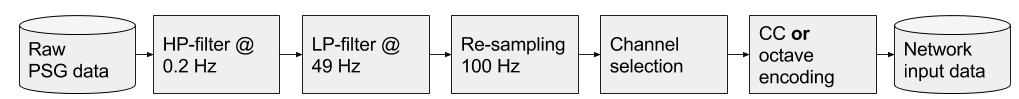
\includegraphics[width=\textwidth]{figures/paper-iii/Figure_5a.png}}  \\
    \subfloat[]
    {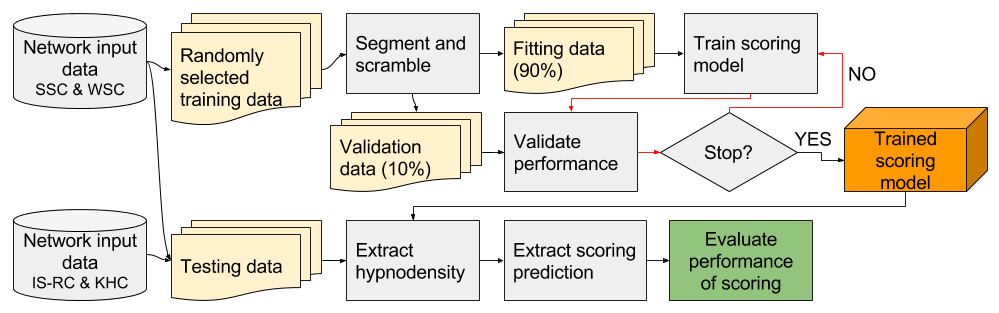
\includegraphics[width=\textwidth]{figures/paper-iii/Figure_5b.png}}
    \caption[STAGES model for sleep staging]{Overview of STAGES model for sleep stage classification. (a) Pre-processing steps taken to achieve the format of data as it is used in the neural networks. One of the 5 channels is first high-pass filtered with a cut-off at 0.2 Hz, then low-pass filtered with a cut-off at 49 Hz followed by a re-sampling to 100 Hz to ensure data homogeneity. In the case of EEG signals, a channel selection is employed to choose the channel with the least noise. The data are then encoded using either the CC or the octave encoding. (b) Steps taken to produce and test the automatic scoring algorithm. A part of the SSC10, 32 and WSC32, 33 is randomly selected, as described in~\cref{tab:paperiii-table01}. These data are then segmented in 5 min segments and scrambled with segments from other subjects to increase batch similarity during training. A neural network is then trained until convergence (evaluated using a separate validation sample). Once trained, the networks are tested on a separate part of the SSC and WSC along with data from the IS-RC31 and KHC10, 34.}
    \label{fig:paperiii-figure05}
\end{figure}
\subsubsection{Datasets}
The success of machine learning depends on the size and quality of the data on which the model is trained and evaluated~\cite{Banko2001, Shotton2011}.
We used a large dataset comprised of several thousand sleep studies to train, validate, and test/replicate our models.
To ensure significant heterogeneity, data came from 10 different cohorts recorded at 12 sleep centers across 3 continents: SSC~\cite{Andlauer2013, Moore2014}, WSC~\cite{Moore2014, Young2009a}, IS-RC~\cite{Kuna2013}, JCTS~\cite{InternationalXyremStudyGroup2005}, KHC~\cite{Hong2006}, AHC~\cite{Frauscher2013}, IHC~\cite{Pizza2015}, DHC~\cite{Christensen2017}, FHC, and CNC~\cite{Andlauer2012}.
Institutional Review Boards approved the study and informed consent was obtained from all participants.
Technicians trained in sleep scoring manually labeled all sleep studies.
Figure 5 a, b, and c summarize the overall design of the study for sleep stage scoring and narcolepsy biomarker development.
\Cref{tab:paperiii-table01} provides a summary of the size of each cohort and how it was used.
In the narcolepsy biomarker aspect of the study, PSGs from T1N and other patients were split across most datasets to ensure heterogeneity in both the training and testing dataset.
For this analysis, a few recordings with poor quality sleep studies, i.e. missing critical channels, with additional sensors or with a too short sleep duration ($\leq$ 2 hours) were excluded.
A “never seen” subset cohort that included French and Chinese subjects (FHC and CNC) was also tested.
Below is a brief description of each dataset.

\paragraph{Population-based Wisconsin Sleep Cohort}
This cohort is a longitudinal study of state agency employees aged 37 - 82 years from Wisconsin, and approximates a population-based sample (see~\cref{tab:paperiii-table01} for age at study) and are generally more overweight33.
The study is ongoing, and dates to 1988.
2167 PSGs in 1086 subjects were used for training while 286 randomly selected PSGs were used for validation testing of the sleep stage-scoring algorithm and narcolepsy biomarker training.
Approximately 25\% of the population have an Apnea Hypopnea Index (AHI) above 15/hour and 40\% have a PLMI above 15/hr.
A detailed description of the sample can be found in Young33 and Moore et al.32.
The sample does not contain any T1N patients, and the three subjects with possible T1N were removed54.

\paragraph{Patient-based Stanford Sleep Cohort}
PSGs from this cohort were recorded at the Stanford Sleep Clinic dating back to 1999, and represent sleep disorder patients aged 18-91 visiting the clinic (see~\cref{tab:paperiii-table01} for age at study).
The cohort contains thousands of PSG recordings, but for this study we used 894 diagnostic (no positive airway pressure (PAP)) recordings in independent patients that have been used in prior studies30.
This subset contains patients with a range of different diagnoses including: sleep disordered breathing (607), insomnia (141), REM sleep behavior disorder (4), restless legs syndrome (23), T1N (25), delayed sleep phase syndrome (14), and other conditions (39).
Description of the subsample can be found in Andlauer et al.10 and Moore et al.32.
Approximately 30\% of subjects have an AHI above 15/hour, or a PLMI above 15/hour.
617 randomly selected subjects were used for training the neural networks while 277 randomly selected PSGs were kept for validation testing of the sleep stage scoring algorithm.
These 277 subjects were also used for training the narcolepsy biomarker algorithm.
The sample contains PSGs of 25 independent untreated subjects with T1N (12 with low CSF hypocretin-1, the others with clear cataplexy).
26 subjects were removed from the study—4 due to poor data quality, and the rest because of medication use.

\paragraph{Patient-based Korean Hypersomnia Cohort}
The Korean Hypersomnia Cohort is a high pretest probability sample for narcolepsy.
It includes 160 patients with a primary complaint of excessive daytime sleepiness (see~\cref{tab:paperiii-table01} for age at study).
These PSGs were used for testing the sleep scoring algorithm and for training the narcolepsy biomarker algorithm.
No data was used for training the sleep-scoring algorithm.
Detailed description of the sample can be found in Hong et al.34 and Andlauer et al.10
The sample contains PSGs of 66 independent untreated subjects with T1N and clear cataplexy.
Two subjects were removed from the narcolepsy biomarker study because of poor data quality.

\paragraph{Patient-based Austrian Hypersomnia Cohort}
Patients in this cohort were examined at the Innsbruck Medical University in Austria as described in Frauscher et al.35.
The AHC contains 118 PSGs in 86 high pretest probability patients for narcolepsy (see~\cref{tab:paperiii-table01} for details).
42 patients (81 studies) are clear T1N with cataplexy cases, with all but 3 having a positive MSLT (these three subjects had a mean sleep latency (MSL)>8 minutes but multiple SOREMPs).
The rest of the sample has idiopathic hypersomnia and type 2 narcolepsy.
Four patients have an AHI>15/hour and 25 had a PLMI>15/hour.
Almost all subjects had two sleep recordings performed, which were kept together such that no two recordings from the same subject were split between training and testing partitions.

\paragraph{Patient-based Inter-scorer Reliability Cohort}
As Rosenberg et al.16 have shown, variation between individual scorers can sometimes be large, leading to an imprecise gold standard.
To quantify this, and to establish a more accurate gold standard, 10 scorers from five different institutions, University of Pennsylvania, St. Luke’s Hospital, University of Wisconsin at Madison, Harvard University, and Stanford University, analyzed the same 70 full night PSGs.
For this study, scoring data from University of Pennsylvania, St. Luke’s and Stanford were used.
All subjects are female (see~\cref{tab:paperiii-table01} for details).
This allowed for a much more precise gold standard, and the inter-scorer reliability could be quantified for a dataset, which could also be examined by automatic scoring algorithms.
Detailed description of the sample can be found in Kuna et al.31 and Malhotra6.
The sample does not contain any T1N patients.

\paragraph{The Jazz Clinical Trial Sample}
This sample includes seven baseline sleep PSGs from five sites taken from a clinical trial study of sodium oxybate in narcolepsy (SXB15 with 45 sites in Canada, USA, and Switzerland) conducted by Orphan Medical, now named Jazz Pharmaceuticals.
The few patients included are those with clear and frequent cataplexy (a requirement of the trial) that had no stimulant or antidepressant treatment at baseline43.
All 7 subjects in this sample were used exclusively for training the narcolepsy biomarker algorithm.

\paragraph{Patient-based Italian Hypersomnia Cohort}
Patients in this high pretest probability cohort (see~\cref{tab:paperiii-table01} for demographics) were examined at the IRCCS, Istituto delle Scienze Neurologiche ASL di Bologna in Italy as described in Pizza et al.41.
The IHC contains 70 \ntI patients (\SI{58}{\percent} male, \plusminus{29.5}{1.9} years old), with either documented low CSF hypocretin levels (59 cases, all but 2 HLA DQB1*06:02 positive), or clear cataplexy, positive MSLTs and HLA positivity (11 subjects).
As non-\ntI cases with unexplained daytime somnolence, the cohort includes 77 other patients: 19 with idiopathic hypersomnia, 7 with type 2 narcolepsy and normal CSF hypocretin-1, 48 with a subjective complaint of excessive daytime sleepiness not confirmed by MSLT, and 3 with secondary hypersomnia.
Subjects in this cohort were used for training (n=87) and testing (n=61) the narcolepsy biomarker algorithm. 

\paragraph{Patient-based Danish Hypersomnia Cohort}
Patients in this cohort were examined at the Rigshospitalet, Glostrup, Denmark as described in Christensen et al53.
The DHC contains 79 PSGs in controls and patients (see~\cref{tab:paperiii-table01} for details).
Based on PSG, multiple sleep latency test and cerebrospinal fluid hypocretin-1 measures, the cohort includes healthy controls (19 subjects), patients with other sleep disorders and excessive daytime sleepiness (20 patients with CSF hypocretin-1 $\geq$ 110 pg/ml), narcolepsy type 2 (22 patients with CSF hypocretin-1 $\geq$ 110 pg/ml), and T1N (28 patients with CSF hypocretin 1 $\leq$ 110 pg/ml).
All 79 subjects in this cohort were used exclusively for training the narcolepsy biomarker algorithm.

\paragraph{Patient-based French Hypersomnia Cohort}
This cohort consists of 122 individual PSGs recorded at the Sleep-Wake Disorders Center, Department of Neurology, Gui-de-Chauliac Hospital, CHU Montpellier, France (see~\cref{tab:paperiii-table01} for demographics).
The FHC contains 63 subjects with T1N (all but two tested with CSF hypocretin-1 $\leq$ 110 pg/ml, five below 18 years old, 55 tested for HLA, all positive for HLA DQB1*06:02) and 22 narcolepsy type 2 (19 with CSF hypocretin-1 > 200 pg/ml, and three subjects with CSF hypocretin-1 between 110 and 200 pg/ml, three HLA positive).
The remaining 36 subjects are controls (15 tested for HLA, two with DQB1*06:02) without other symptoms of hypersomnia.
The FHC was used as data for the replication study of the narcolepsy biomarker algorithm.

\paragraph{Patient-based Chinese Narcolepsy Cohort}
This cohort contains 199 individual PSGs recorded (see~\cref{tab:paperiii-table01} for demographics).
The CNC contains 67 subjects diagnosed with T1N exhibiting clear-cut cataplexy (55 tested HLA DQB1*06:02 positive), while the remaining 132 subjects are randomly selected population controls (15 HLA DQB1*06:02 positive, 34 HLA negative, remaining unknown) 12.
Together with the FHC, the CNC was used as data for the replication study of the narcolepsy biomarker algorithm.

\paragraph{American Academy of Sleep Medicine Sleep Study}
The AASM ISR dataset is composed of a single control sleep study of 150 30 sec epochs that was scored by \plusminus{5234}{14} experienced sleep technologists for quality control purposes.
Design of this dataset is described in Rosenberg et al.16.

\subsubsection{Data labels, scoring and fuzzy logic}
Sleep stages were scored by PSG-trained technicians using established scoring rules, as described in the AASM Scoring Manual7.
In doing so, technicians assign each epoch with a discrete value.
With a probabilistic model, like the one proposed in this study, a relationship to one of the fuzzy sets is inferred based on thousands of training examples labeled by many different scoring-technicians. 

The hypnodensity graph refers to the probability distribution over each possible stage for each epoch, as seen in Figure 2 a and b.
This allows more information to be conveyed, since every epoch of sleep within the same stage is not identical. For comparison with the gold standard, however, a discrete value must be assigned from the model output as:

\begin{equation}
    \hat{y} = \argmax_{\mathbf{y}_{i}} \sum_{i}^{N} \mathbf{P}_i \! \left( \mathbf{y}_i \! \mid \! \mathbf{x}_i \right),
\end{equation}
where $\mathbf{P}_i \! \left( \mathbf{y}_i \! \mid \! \mathbf{x}_i \right)$ is a vector with the estimated probabilities for each sleep stage in the \textit{i}th segment, $N$ is the number of segments an epoch is divided into, and $\hat{y}$ is the estimated label. 

Sleep scoring technicians score sleep in 30 second epochs, based on what stage they assess is represented in the majority of the epoch—a relic of when recordings were done on paper. This means that when multiple sleep stages are represented, more than half of the epoch may not match the assigned label. This is evident in the fact that the label accuracy decreases near transition epochs20. One solution to this problem is to remove transitional regions to purify each class. However, this has the disadvantage of under-sampling transitional stages, such as N1, and removes the context of quickly changing stages, as is found in a sudden arousal. It has been demonstrated that the negative effects of imperfect “noisy” labels may be mitigated if a large enough training dataset is incorporated and the model is robust to overfitting41. This also assumes that the noise is randomly distributed with an accurate mean—a bias cannot be cancelled out, regardless of the amount of training data. For these reasons, all data including those containing sleep transitions were included. Biases were evaluated by incorporating data from several different scoring experts cohorts and types of subjects.

To ensure quick convergence, while also allowing for long-term dependencies in memory-based models, the data were broken up in 5 minute blocks and shuffled to minimize the shift in covariates during training caused by differences between subjects. To quantify the importance of segment sizes, both 5 second and 15 second windows were also tested.

\begin{landscape}
\begin{table}
\begin{threeparttable}  
\centering
\small
\caption[STAGES cohorts]{Description of the various cohorts included in this study and how they were used.}
\label{tab:paperiii-table01}
\begin{tabular}{@{}lccccccccccc@{}}
    \toprule
    & & & & \multicolumn{2}{c}{Sleep scoring} & \multicolumn{3}{c}{Narcolepsy biomarker} & & & \\ \cline{5-6} \cline{7-9}
    Cohort         & Age, $ \mu \pm \sigma $        & BMI, $ \mu \pm \sigma $        & Sex, \% male       & Train      & Test      & Train  & Test              & Replication            & \% narco & \% hypersomnia \\ \midrule
    WSC            & 59.7 $ \pm $ 8.4  & 31.6 $ \pm $ 7.1  & 53.1      & 1086 (2167~PSGs) & 286  & 170                  & 116          & None        & 0        & 0 \\
    SSC            & 45.4 $ \pm $ 13.8 & 23.9 $ \pm $ 6.5  & 59.4      & 617                & 277  & 139                  & 112          & None        & 11.6     & 1.8 \\
    KHC            & 29.1 $ \pm $ 13.2 & 24.1 $ \pm $ 4.3  & 58.6      & None               & 160  & 87                   & 71           & None        & 45.8     & 54.2 \\
    AHC            & 34.5 $ \pm $ 13.8 & 25.9 $ \pm $ 4.9  & 54        & None               & None & 42 (76~PSGs)         & 44 (84~PSGs) & None        & 52.3     & 47.7 \\
    IS-RC          & 51.1 $ \pm $ 4.2  & 32.9 $ \pm $ 9.2  & 0         & None               & 70   & None                 & None         & None        & 0        & 0 \\
    JCTS           & 53.2 $ \pm $ 9.8  & 31.0 $ \pm $ 4.4  & 57.1      & None               & None & 7                    & None         & None        & 100      & 0 \\
    IHC            & 33.7 $ \pm $ 17.6 & -           & 56.7      & None               & None & 87                   & 61           & None        & 47.3     & 50 \\
    DHC            & 33.4 $ \pm $ 14.8 & 24.8 $ \pm $ 4.9  & 50        & None               & None & 79                   & None         & None        & 26.6     & 48.1 \\
    FHC            & 28.8 $ \pm $ 15.2 & 24.4 $ \pm $ 8.1  & 59        & None               & None & None                 & None         & 122         & 51.6     & 18 \\
    CNC            & 28.5 $ \pm $ 16.9 & 23.2 $ \pm $ 11.5 & 51.3      & None               & None & None                 & None         & 199         & 34.2     & 0 \\ \midrule
    Total subjects &             &             &           & 1,703              & 793  & 611                  & 404          & 321         &          & \\
    Total PSGs     &             &             &           & 2,784              & 793  & 645                  & 444          & 321         &          & \\ \bottomrule
\end{tabular}
\begin{tablenotes}
\footnotesize
\item WSC, SSC \quad Training and testing of sleep scoring models and narcolepsy biomarker.
\item KHC \quad Sleep scoring testing, and training and testing of narcolepsy biomarker.
\item AHC \quad Training and testing of narcolepsy biomarker. 86 subjects had the first PSG recorded, and 75 had an additional second PSG.\newline A subject was used for either training or testing.
\item IS-RC \quad Scored by 6 different scorers. Final assessment and validation of predictive performance for sleep scoring.
\item JCTS, DHC \quad Training of narcolepsy biomarker.
\item IHC \quad Training and testing of narcolepsy biomarker.
\item FHC, CNC \quad Replication of narcolepsy biomarker. 
\end{tablenotes}
\end{threeparttable}
\end{table}
\end{landscape}

\subsubsection{Data selection and pre-processing}
A full night PSG involves recording many different channels, some of which are not necessary for sleep scoring55. In this study, EEG – C3 or C4, and O1 or O2, chin EMG, and the left and right EOG channels were used, with reference to the contralateral mastoid. Poor electrode connections are common when performing a PSG analysis. This can lead to a noisy recording, rendering it useless. To determine whether right or left EEG channels were used, the noise of each was quantified by dividing the EEG data in 5 minute segments, and extracting the Hjorth parameters56. These were then log-transformed, averaged, and compared with a previously established multivariate distribution, based on the WSC32,33 and SSC10,32 training data. The channel with lowest Mahalanobis distance57 to this distribution was selected. The log-transformation has the advantage of making flat signals/disconnects as uncommon as very noisy signals, in turn making them less likely to be selected. To minimize heterogeneity across recordings, and at the same time reducing the size of the data, all channels were down-sampled to 100 Hz. Additionally, all channels were filtered with a 5th order two-direction infinite impulse response (IIR) high-pass filter with cutoff frequency of 0.2 Hz and a 5th order two-direction IIR low-pass filter with cutoff frequency of 49 Hz. The EMG signal contains frequencies well above 49 Hz, but since much data had been down-sampled to 100 Hz in the WSC, this cutoff was selected for all cohorts. All steps of the pre-processing are illustrated in Figure 5 a.

\subsubsection{Convolutional and recurrent neural networks}
Convolutional neural networks (CNN) are a class of deep learning models first developed to solve computer vision problems30. A CNN is a supervised classification model in which a low-level, such as an image, is transformed through a network of filters and sub-sampling layers. Each layer of filters produces a set of features from the previous layer, and as more layers are stacked, more complex features are generated. This network is coupled with a general-purpose learning algorithm, resulting in features produced by the model reflecting latent properties of the data rather than the imagination of the designer. This property places fewer constrictions on the model by allowing more flexibility, and hence the predictive power of the model will increase as more data is observed. This is facilitated by the large number of parameters in such a model, but may also necessitate a large amount of training data. Sleep stage scoring involves a classification of a discrete time-series, in which adjacent segments are correlated. Models that incorporate memory may take advantage of this and may lead to better overall performance by evening out fluctuations. However, these fluctuations may be the defining trait or anomaly of some underlying pathology (such as narcolepsy, a pathology well known to involve abnormal sleep stages transitions), present in only a fraction of subjects, and perhaps absent in the training data. This can be thought of similarly to a person with a speech impediment: the contextual information will ease the understanding, but knowing only the output, this might also hide the fact that the person has such a speech impediment. To analyze the importance of this, models with and without memory were analyzed. Memory can be added to such a model by introducing recurrent connections in the final layers of the model. This turns the model into a recurrent neural network (RNN). Classical RNNs had the problem of vanishing or exploding gradients, which meant that optimization was very difficult. This problem was solved by changing the configuration of the simple hidden node into a LSTM cell58. Models without this memory are referred to as FF models. A more in-depth explanation of CNNs including application areas can be found the review article on deep learning by LeCun, Bengio and Hinton30 and the deep learning textbook by Goodfellow, Bengio and Courville (2016)59. For a more general introduction to machine learning concepts, see the textbook by Bishop (2006)60.

\subsubsection{Data input and transformations}
Biophysical signals, such as those found in a PSG, inherently have a low signal to noise ratio, the degree of which varies between subjects, and hence learning robust features from these signals may be difficult. To circumvent this, two representations of the data that could minimize these effects were selected. An example of each decomposition is shown in~\cref{fig:paperiii-figure06}.

\begin{figure}[!tb]
    \myfloatalign   
    \subfloat[]
    {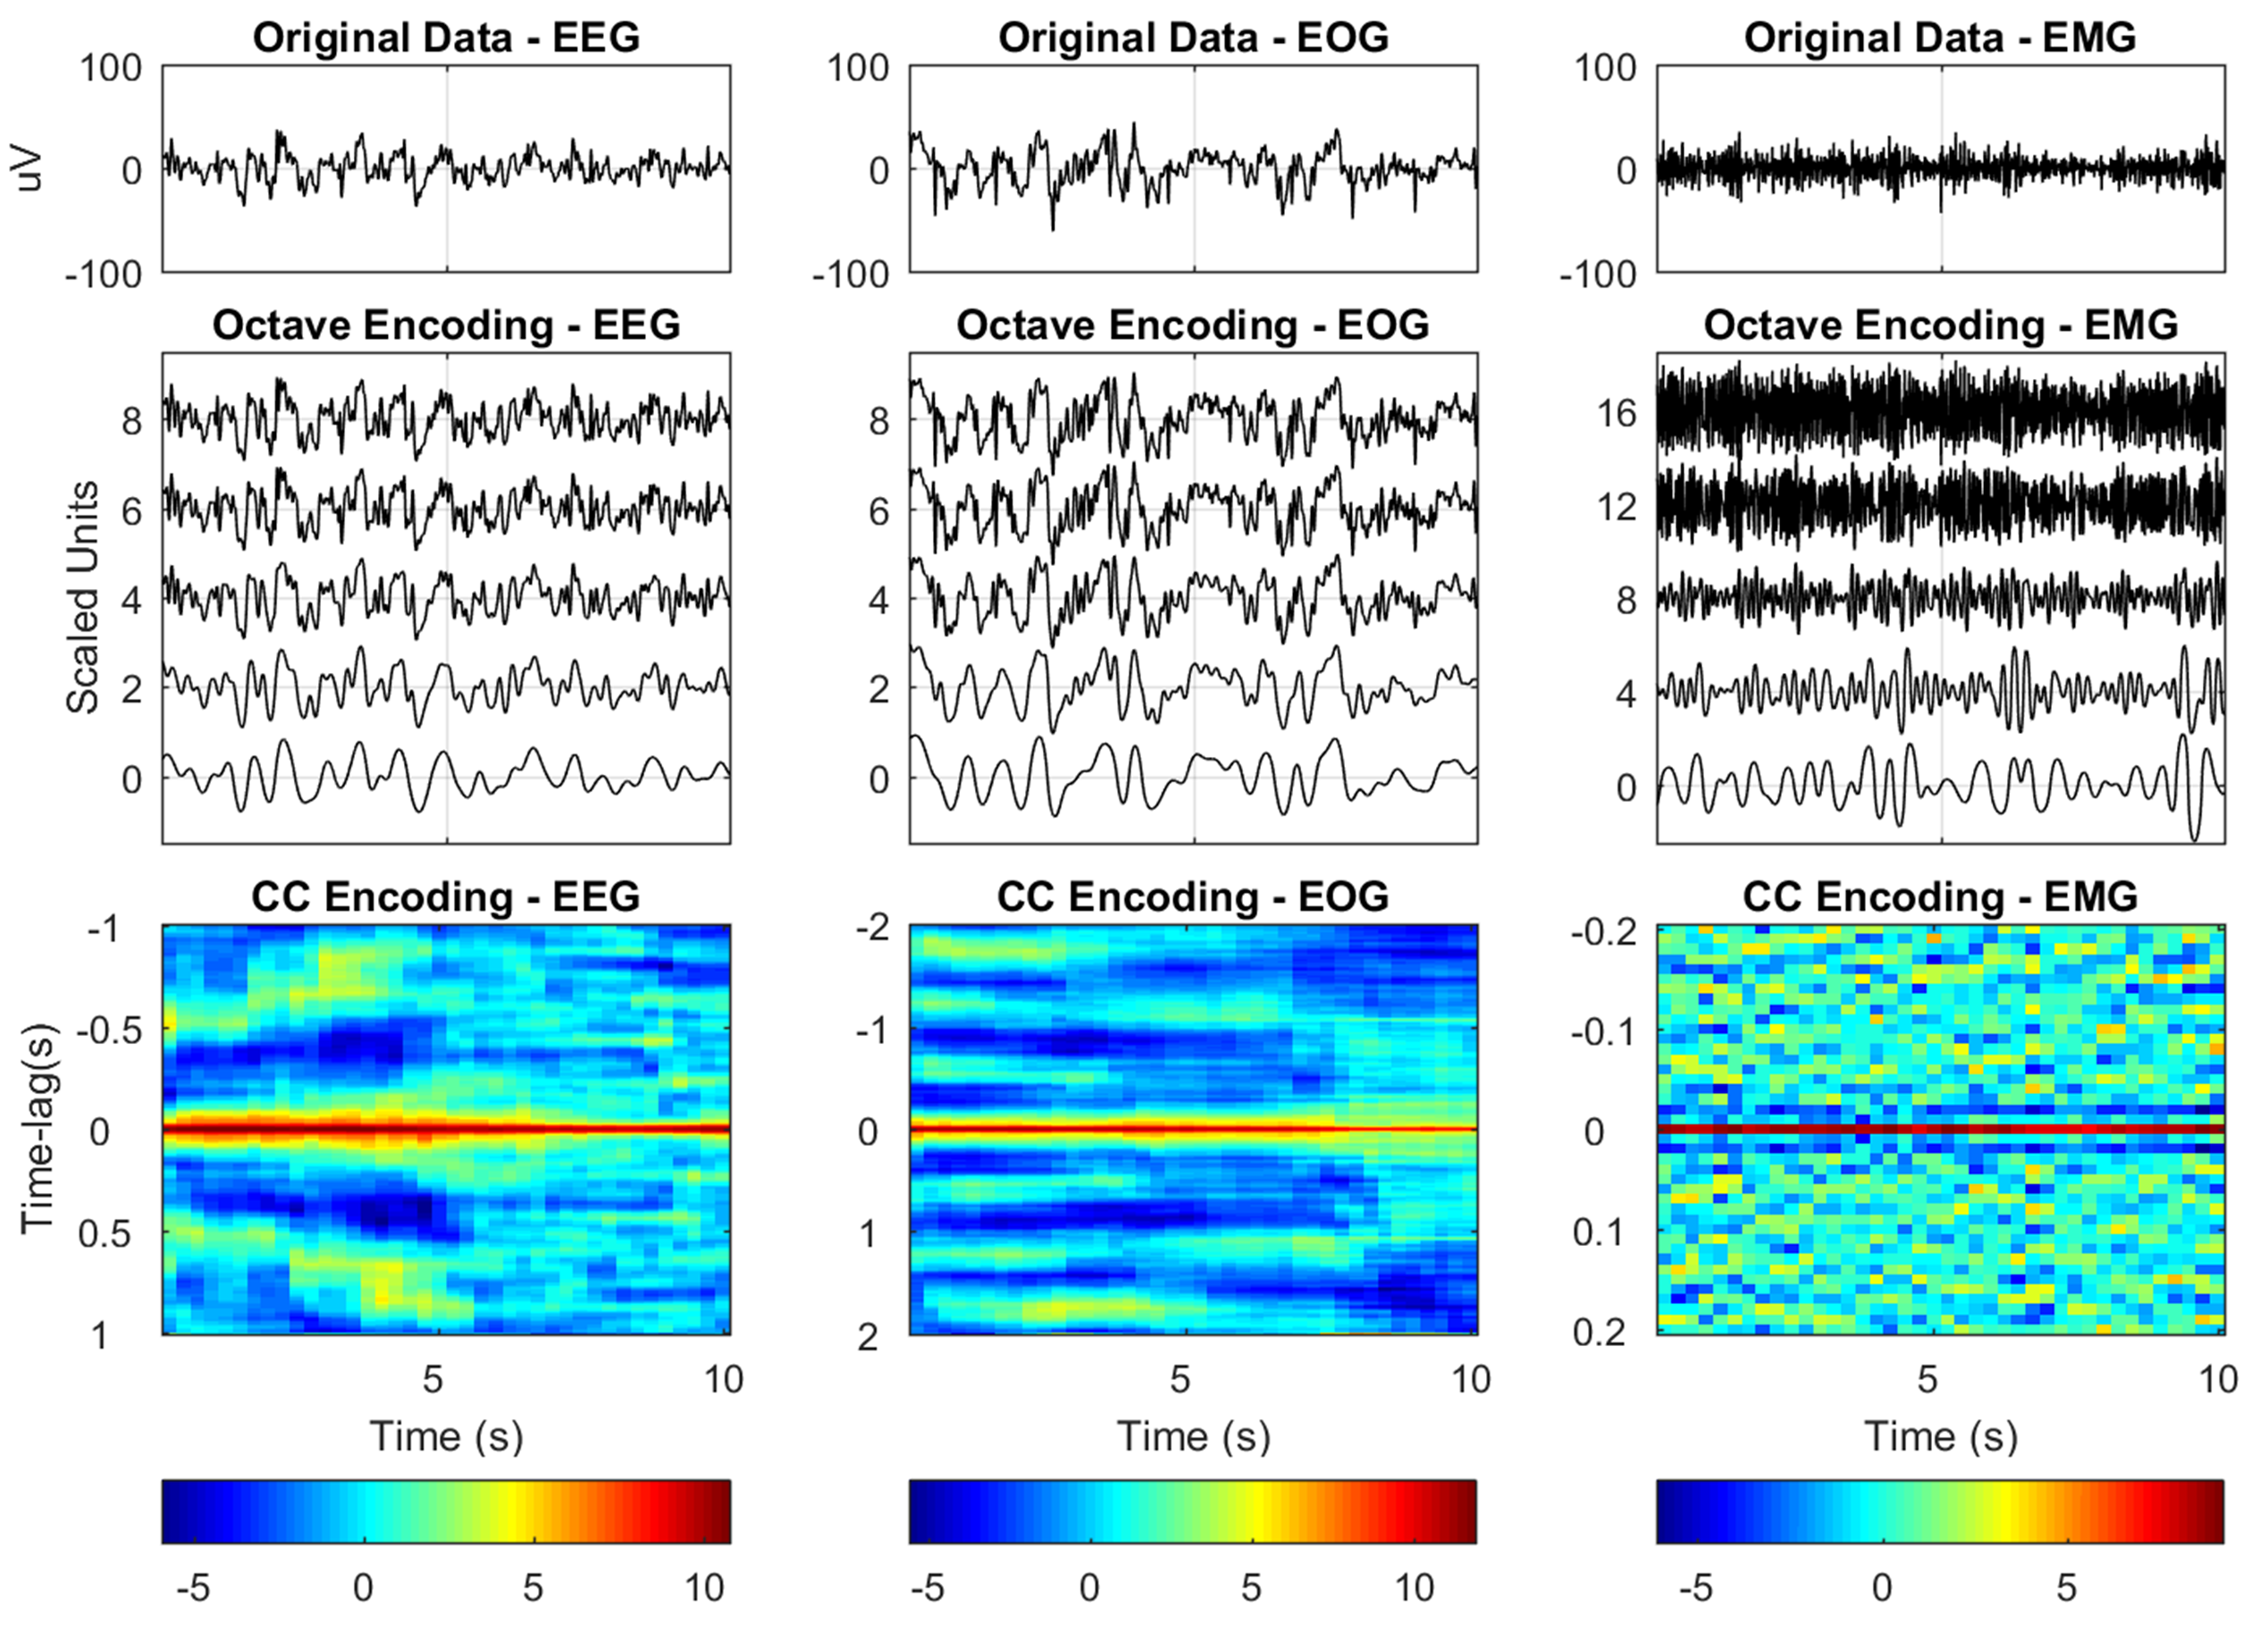
\includegraphics[width=\textwidth]{figures/paper-iii/ncomm_figure6a-2}}  \\
    \subfloat[]
    {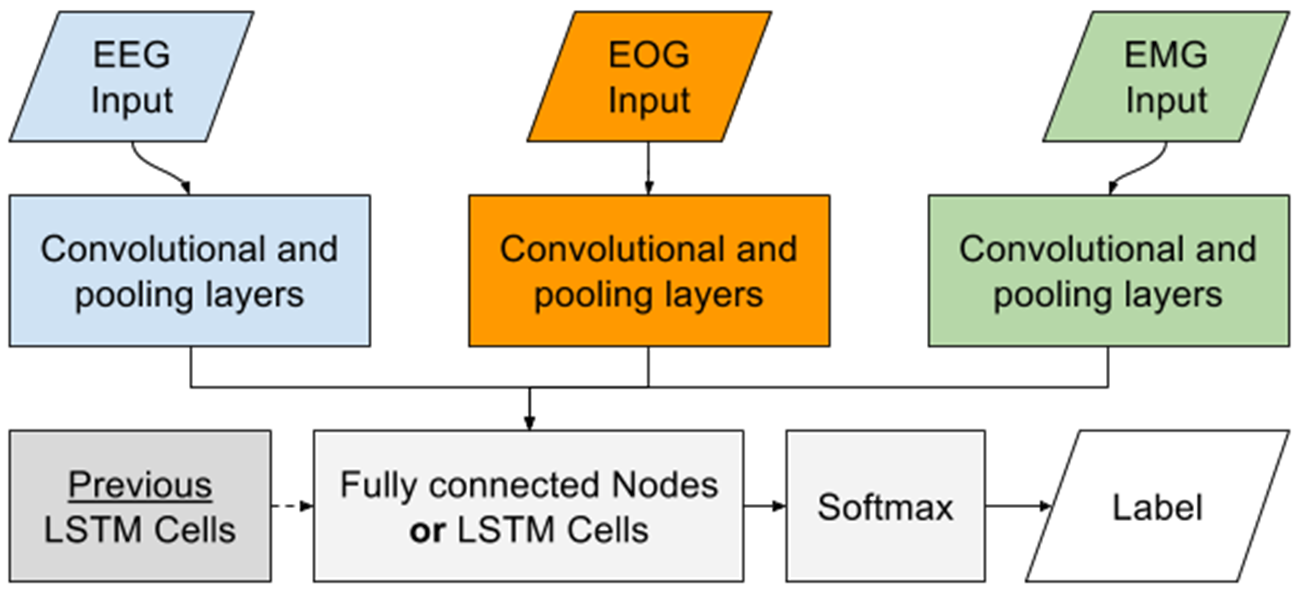
\includegraphics[width=0.7\textwidth]{figures/paper-iii/ncomm_figure6b-2}}
    \caption[Neural network strategy for STAGES model]{Neural network strategy for STAGES model. (a) An example of the octave and the CC encoding on 10 s of EEG, EOG and EMG data. These processed data are fed into the neural networks in one of the two formats. The data in the octave encoding are offset for visualization purposes. Color scale is unitless. (b) Simplified network configuration, displaying how data are fed and processed through the networks. A more detailed description of the network architecture is shown in~\cref{fig:paperiii-suppfigure03}.}
    \label{fig:paperiii-figure06}
\end{figure}

Octave encoding maintains all information in the signal, and enriches it by repeatedly removing the top half of the bandwidth (i.e. cut off frequencies of \SIlist{49;25;12.5;6.25;3.125}{\hertz}) using a series of low-pass filters, yielding a total of 5 new channels for each original channel. At no point is a high-pass filter applied. Instead, the high frequency information may be obtained by subtracting lower frequency channels —– an association the neural networks can make, given their universal approximator properties61. After filtration, each new channel is scaled to the 95th percentile and log modulus transformed:
\begin{equation}
    \mathbf{x}_{\mathrm{scaled}} = \sign \! \left( \mathbf{x} \right) \log{\left( \frac{|\mathbf{x}|}{p_{95}(\mathbf{x})} + 1 \right)}
\end{equation}
The initial scaling places 95\% of the data between -1 and 1, a range in which the log modulus is close to linear. Very large values, such as those found in particularly noisy areas, are attenuated greatly. Some recordings are noisy, making the \nth{95} percentile significantly higher than what the physiology reflects. Therefore, instead of the selecting the \nth{95} percentile from the entire recording, the recording is separated into 50\% overlapping 90 minute segments, from which the 95th percentile is extracted. The mode of these values is then used as a scaling reference. In general, scaling and normalization is important to ensure quick convergence as well as generalization in neural networks. The decomposition is done in the same way on every channel, resulting in 25 new channels in total.

Using a cross-correlation function, underlying periodicities in the data are revealed while noise is attenuated. White noise is by definition uncorrelated; its autocorrelation function is zero everywhere except lag zero. It is this property that is utilized, even though noise cannot always be modeled as such. PSG signals are often obscured by undesired noise that is uncorrelated with other aspects of the signals. An example CC between a signal segment and an extended version of the same signal segment is shown in~\cref{fig:paperiii-suppfigure05}. Choosing the CC in this manner over a standard autocorrelation function serves two purposes: the slow frequencies are expressed better, since there is always full overlap between the two signals (some of this can be adjusted with the normal autocorrelation function using an unbiased estimate); and the change in fluctuations over time within a segment is expressed, making the function reflect aspects of stationarity. Because this is the CC between a signal and an extended version of itself, the zero lag represents the power of that segment, as is the case in an autocorrelation function.
\begin{figure}[tb]
    \centering
    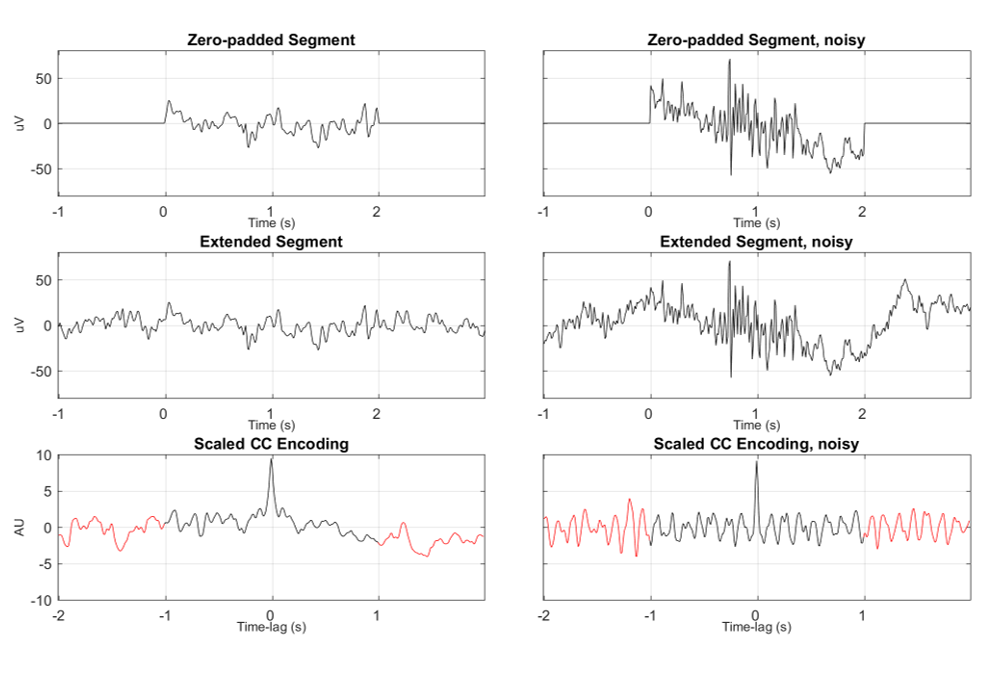
\includegraphics[width=\textwidth]{figures/paper-iii/SuppFigure_5.png}
    \caption{}
    \label{fig:paperiii-suppfigure05}
\end{figure}

Frequency content with a time resolution may also be expressed using time-frequency decompositions, such as spectrograms or scalograms, however, one of the key properties of a CNN is the ability to detect distinct features anywhere in an input, given its property of equivariance62. A CC function reveals an underlying set of frequencies as an oscillation pattern, as opposed to a spectrogram, where frequencies are displayed as small streaks or spots in specific locations, corresponding to frequencies at specific times. The length and size of each CC reflects the expected frequency content and the limit of quasi-stationarity (i.e. how quickly the frequency content is expected to change).

The EOG signal reveals information about eye movements such as REMs, and to some extent EEG activity6,7. In the case of the EOG signal, the relative phase between the two channels is of great importance to determine synchronized eye movements, and hence a CC of opposite channels (i.e. either the extended or zero padded signal is replaced with the opposite channel) is also included. The slowest eye-movements happen over the course of several seconds6,7, and hence a segment length of 4 seconds was selected for the correlation functions. To maintain resolution flexibility with the EEG, an overlap of 3.75 seconds was chosen.

In the case of the EMG signal, the main concern is the signal amplitude and the temporal resolution, not the actual frequencies. As no relevant low frequency content is expected, a segment length of 0.4 seconds and an overlap of 0.25 seconds was selected.

As with the octave encoding, the data is scaled, although only within segments:
\begin{equation}
    D_i = \frac{ \gamma_{\mathbf{x}_i \mathbf{y}_i} \func{\log}{1 + \func{\max}{\left|\gamma_{\mathbf{x}_i \mathbf{y}_i}\right|}}}{\func{\max}{\left|\gamma_{\mathbf{x}_i \mathbf{y}_i}\right|}}
\end{equation}
where $D_i$ is the scaled correlation function and $\gamma_{\mathbf{x}_i \mathbf{y}_i}$ is the unscaled correlation function.

\subsubsection{Architectures of applied CNN models}
\begin{figure}[tb]
    \centering
    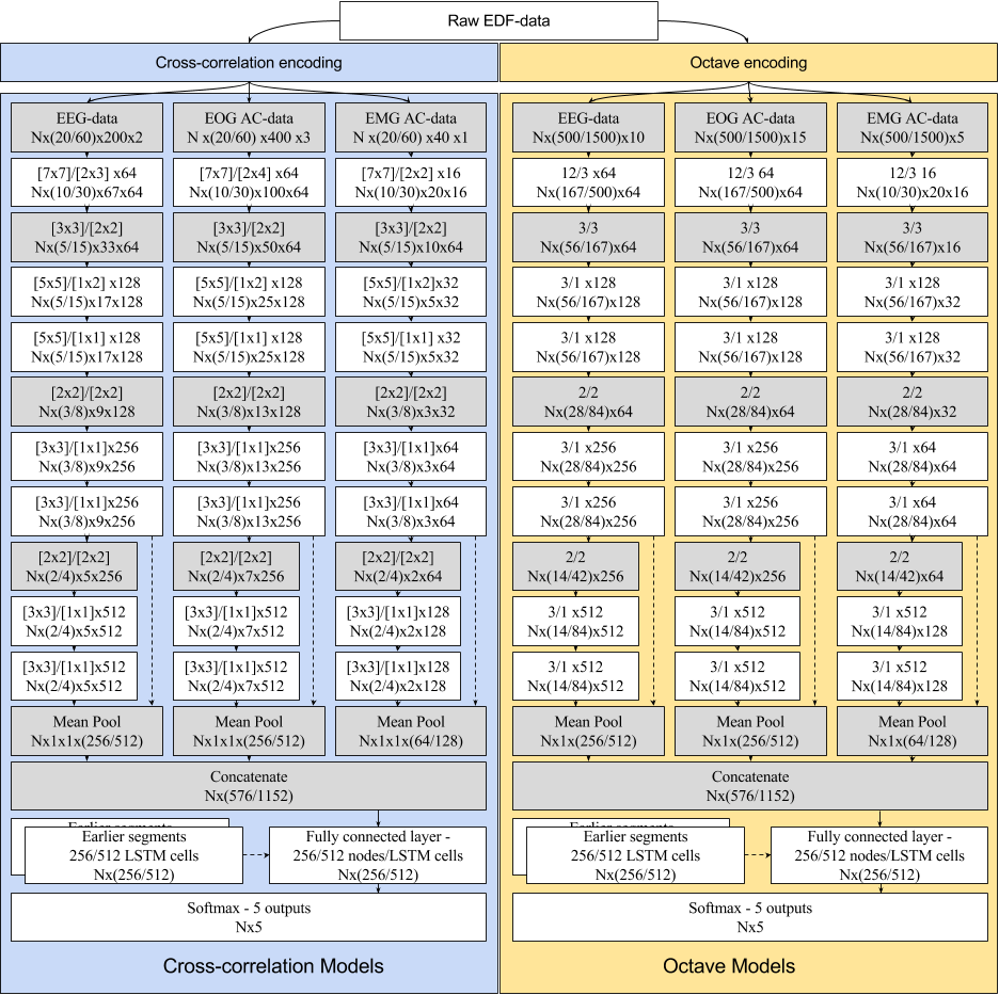
\includegraphics[width=\textwidth]{figures/paper-iii/SuppFigure_3.png}
    \caption{Caption}
    \label{fig:paperiii-suppfigure03}
\end{figure}
The architecture of a CNN typically reflects the complexity of the problem that is being solved and how much training data is available, as a complex model has more parameters than a simple model, and is therefore more likely to over-fit. However, much of this may be solved using proper regularization. Another restriction is the resources required to train a model—deep and complex models require far more operations and will therefore take longer to train and operate. In this study, no exhaustive hyper-parameter optimization was carried out. The applied architectures were chosen on the basis of other published models63. Since the models utilized three separate modalities (EEG, EOG and EMG), three separate sub-networks were constructed. These were followed by fully connected layers combining the inputs from each sub-network, which were passed onto a softmax output (Figure 6 b, Supplementary Figure 3). Models that utilize memory have fully connected hidden units replaced with LSTM cells and recurrent connections added between successive segments. Networks of two different sizes are evaluated to quantify the effect of increasing complexity. 

\subsubsection{Training of CNN models}
Training the models involves optimizing parameters to minimize a loss function evaluated across a training dataset. The loss function was defined as the cross-entropy with L2 regularization:
\begin{align}
\begin{split}
    L(\boldsymbol{\omega}) &= \frac{1}{N}\sum_{i=1}^{N} \func{H}{\mathbf{y}_i, \hat{\mathbf{y}}_i} + \ell_2 \\
    &= \frac{1}{N}_{i=1}^{N} \mathbf{y}_i \func{\log}{\hat{\mathbf{y}}_i} + \left( 1 - \mathbf{y}_i \right) \func{\log}{1 - \hat{\mathbf{y}}_i} + \lambda \| \boldsymbol{\omega} \|^2_2,
\end{split}
\end{align}
where $\mathbf{y}_i$ is the true class label of the \textit{i}th window, $\hat{\mathbf{y}}_i$ is the estimated probability of the \textit{i}th window, $\omega$ is the parameter to be updated, and $\lambda$ is the weight decay parameter set at $10^{-5}$. The model parameters were initialized with $\func{\mathcal{N}}{0, 0.01}$, and trained until convergence using stochastic gradient decent with momentum64. Weight updates were done as: $\boldsymbol{\omega}_{t+1} = \boldsymbol{\omega}_t + \eta \mathbf{v}_{t+1}$ with $\mathbf{v}_{t+1} = \alpha \mathbf{v}_t - \frac{\partial \mathbf{L}}{\partial \boldsymbol{\omega}_t}$, where $\alpha$ is the momentum set at 0.9, $\mathbf{v}_t$ is the learning velocity initialized at 0, and $\eta$ is the learning rate, initially set at 0.005. The learning rate was gradually reduced with an exponential decay $\eta = \eta_0 \exp^{-t/\tau}$, where $t$ is the number of updates and $\tau$ is a time constant, here set to 12.000.

Over-fitting was avoided using a number of regularization techniques, including batch normalization65, weight decay66, and early stopping67. Early stopping is accomplished by scheduling validation after every 50th training batch. This is done by setting aside 10\% of the training data. Training is stopped if the validation accuracy starts to decrease, as a sign of over-fitting. For LSTM networks, dropout68 was included, set at 0.5 while training. This ensured that model parameters generalized to the validation data and beyond. During training, data-batches were selected at random. Given the stochastic nature of the training procedure, it was likely that two realizations of the same model would not lead to the same results, since models end up in different local minima. To measure the effect of this, two realizations were made of each model.

Apart from model realizations, we also investigated the effect of ensembling our sleep stage classification model. In general, ensemble models can yield higher predictive performance than any single model by attacking a classification or regression problem from multiple angles. For our specific use case, this resolves into forming a sleep stage prediction based on the predictions of all the models in the given ensemble. We tested several ensembles containing various numbers of model architectures and data encodings, as described in Supplementary Table 8. 

\subsubsection{Performance comparisons of generated CNN models}
As stated, the influences of many different factors were analyzed. These included: using octave or CC encoding, short (5 s) or long (15 s) segment lengths, low or high complexity, with or without LSTM, and using a single or two realizations of a model. To quantify the effect of each, a $2^5$-factorial experiment was designed. This lead to 32 different models, see~\cref{tab:paperiii-supptable08}. Comparison between models was done on a per epoch basis. 
\begin{table}[tb]
    \centering
    \small
    \caption[STAGES models]{STAGES model tested. 32 single models are tested, and 9 ensembles, totaling 41 models.}
    \label{tab:paperiii-supptable08}
    \begin{tabular}{@{}lllll@{}}
        \toprule
        \multicolumn{5}{c}{Single models} \\ \midrule
        Memory        & Seg. Len. & Complexity & Encoding & Realizations \\
        Simple FF     & 5 s       & Low        & Octave   & 1            \\
        LSTM          & 15 s      & High       & CC       & 2            \\ \bottomrule
    \end{tabular}
    \\
    \small
    \begin{tabular}{@{}llllllllll@{}}
        \toprule
        \multicolumn{10}{c}{Ensembles} \\ \midrule
        Parameters included & All Oct FF & All Oct LSTM & All CC FF & All CC LSTM & All FF & All LSTM & All Oct models & All CC models & All models \\
        N. models           & 8          & 8            & 8         & 8           & 16     & 16       & 16             & 16            & 32         \\ \bottomrule
    \end{tabular}
\end{table}

\subsection{Results}
\subsubsection{Inter-scorer reliability cohort}

\Cref{tab:paperiii-table01} reports on the description of the various cohorts included in this study, and how they were utilized (see Datasets section in Methods).
These originate from seven different countries. 
We assessed inter-scorer reliability using the Inter-scorer Reliability Cohort (IS-RC)31, a cohort of 70 PSGs scored by 6 scorers across three locations in the United States31.
\cref{tab:paperiii-table01} displays individual scorer performance as well as the averaged performance across scorers, with top and bottom of table showing accuracies and \cohen, respectively.
The results are shown for each individual scorer when compared to the consensus of all scorers (biased) and compared to the consensus of the remaining scorers (unbiased).
In the event of no majority vote for an epoch, the epoch was counted equally in all classes in which there was disagreement.
Also shown in~\cref{tab:paperiii-table01} is the model performance on the same consensus scorings as each individual scorer along with the \textit{t}-statistic and associated \textit{p}-value for each paired \textit{t}-test between the model performance and individual scorer performance. 
At a significance level of 5\%, the model performs statistically better than any individual scorer both in terms of accuracy and \cohen.

Supplementary Table 2 displays the confusion matrix for every epoch of every scorer of the inter-scorer reliability data, both unadjusted (top) and adjusted (bottom).
As in Rosenberg and Van Hout16, the biggest discrepancies occur between N1 and Wake, N1 and N2, and N2 and N3, with some errors also occurring between N1 and REM, and N2 and REM.

For future analyses of the IS-RC in combination with other cohorts that have been scored only by one scorer, a final hypnogram consensus was built for this cohort based on the majority vote weighted by the degree of consensus from each voter, expressed as its 
\begin{equation}
    \cohen = 1 + \frac{1 - p_o}{1 - p_e},
\end{equation}
where $p_e$ is the baseline accuracy and $p_o$ is the scorer accuracy, such that
\begin{equation}
    \mathbf{y} = \argmax \frac{\sum_{i=1}^{6} \hat{\mathbf{y}}_i \cdot \boldsymbol{\kappa}_i}{\sum_{i=1}^{6} \boldsymbol{\kappa}_i}
\end{equation}
In this implementation, scorers with a higher consensus with the group are considered more reliable and have their assessments weighted heavier than the rest.
This also avoided split decisions on end-results.
\begin{table}
    \centering
    \caption{Performance of best models, as they are described by supplementary table 2, on various data-sets compared to the six-scorer consensus. All comparisons are on a by-epoch-basis.}
    \label{tab:paperiii-table02}
    \small
    \begin{tabular}{@{}lllll@{}}
        \toprule
        Test Data          & Best Single Model & Acc., \% & Best Ensemble & Acc., \% \\ \midrule
        WSC                & CC/SH/LS/LSTM/2   & $86.0 \pm 5.0$       & All CC        & $86.4 \pm 5.2$       \\
        SSC+KHC & & & & \\
        \quad $\div$ narcolepsy            & CC/LH/SS/LSTM     & $76.9 \pm 11.1$      & All CC        & $77.0 \pm 11.9$      \\
        \quad $+$ narcolepsy & CC/LH/SS/LSTM     & $68.8 \pm 11.0$      & All CC        & $68.4 \pm 12.2$      \\
        IS-RC              & CC/LH/LS/LSTM/2   & $84.6 \pm 4.6$       & All Models    & $86.8 \pm 4.3$       \\ \bottomrule
    \end{tabular}
\end{table}

\begin{landscape}
\begin{table}
    \centering
    \caption[Scorer and model performance]{Individual and overall scorer performance, expressed as accuracy (upper half) and \cohen (lower half). Both accuracy and \cohen are presented with (biased) and without (unbiased) the assessed scorer included in the consensus standard in a leave-one-out fashion. Accuracy is expressed in percent, and \cohen is a ratio and therefore unitless. \textit{t}-statistics and \textit{p}-values correspond to the paired \textit{t}-test between the unbiased predictions for each scorer against the model predictions on the same consensus.}
    \label{tab:paperiii-table01}
    \begin{tabular}{@{}llllllll@{}}
        \toprule
                                           & Overall      & Scorer 1               & Scorer 2               & Scorer 3                & Scorer 4              & Scorer 5               & Scorer 6                \\ \midrule
        Accuracy, \%                       &              &                        &                        &                         &                       &                        &                         \\
        \quad Biased                       & $81.3\pm3.0$ & $82.4\pm6.1$           & $84.6\pm5.5$           & $74.1\pm7.9$            & $85.4\pm5.7$          & $83.1\pm9.4$           & $78.3\pm8.9$            \\
        \quad Unbiased                     & $76.0\pm3.2$ & $77.3\pm6.3$           & $79.1\pm6.3$           & $69.0\pm8.0$            & $79.7\pm6.5$          & $77.8\pm9.6$           & $72.9\pm9.2$            \\
        \quad Model, \%                    & -            & $85.1\pm4.9$           & $83.8\pm5.0$           & $86.5\pm4.3$            & $84.3\pm4.7$          & $85.6\pm4.7$           & $87.0\pm4.5$            \\
        \textit{t}-stat (\textit{p}-value) & -            & $9.5$ ($3.8 \times 10^{-14}$) & $6.6$ ($7.5\times 10^{-9}$)  & $18.3$ ($6.0\times10^{-28}$) & $6.7$ ($4.7\times10^{-9}$) & $6.4$ ($1.7\times10^{-8}$)  & $12.2$ ($7.5\times10^{-19}$) \\ \midrule
        \cohen                             &              &                        &                        &                         &                       &                        &                         \\
        \quad Biased                       & $61.0\pm6.8$ & $63.6\pm12.2$          & $68.4\pm10.5$          & $45.6\pm19.7$           & $69.6\pm13.2$         & $64.5\pm20.9$          & $54.5\pm19.8$           \\
        \quad Unbiased                     & $57.7\pm6.1$ & $61.3\pm11.2$          & $64.6\pm10.3$          & $43.5\pm19.2$           & $64.6\pm13.1$         & $60.9\pm16.9$          & $51.6\pm16.7$           \\
        \quad Model                        & -            & $74.3\pm12.3$          & $72.4\pm12.1$          & $76.0\pm11.8$           & $72.7\pm12.0$         & $74.7\pm12.1$          & $76.6\pm12.2$           \\
        \textit{t}-stat (\textit{p}-value) & -            & $9.5$ ($4.6\times10^{-14}$) & $7.1$ ($7.9\times10^{-10}$) & $15.4$ ($7.0\times10^{-24}$) & $6.6$ ($6.4\times10^{-9}$) & $7.1$ ($9.2\times10^{-10}$) & $13.2$ ($2.0\times10^{-20}$) \\ \bottomrule
    \end{tabular}
\end{table}
\end{landscape}

\begin{figure}
    \centering
    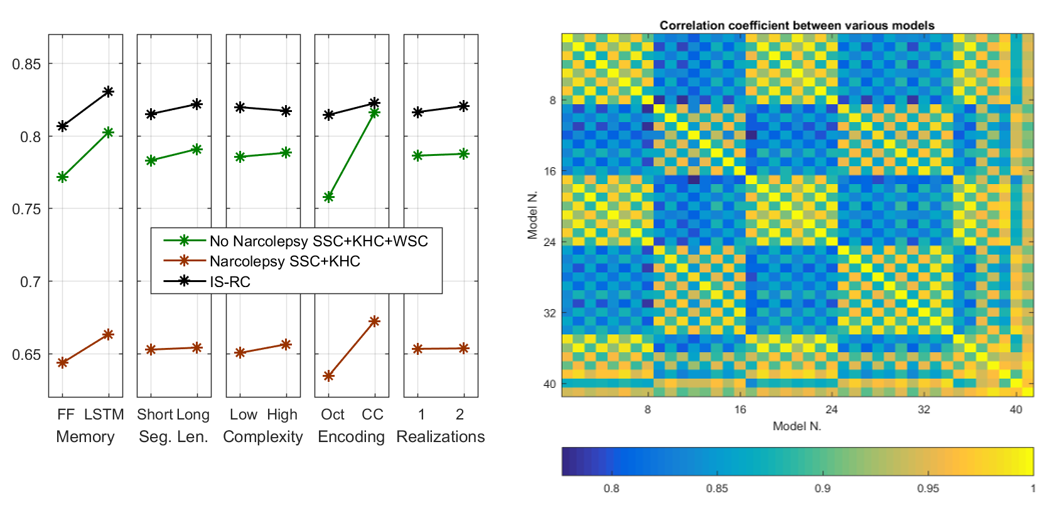
\includegraphics[width=\textwidth]{figures/paper-iii/SuppFigure_1.png}
    \caption[Comparisons of machine learning models]{Comparisons of machine learning models. Left: Comparisons of the effect on accuracy by each factor at different settings on IS-RC data, SSC and KHC narcolepsy subjects, and the remaining SSC, KHC and WSC subjects used for testing. Right: Correlation matrix showing similarities in different model predictions, where 0 means signals are independent, and 1 means signals are completely correlated. Models 1-32 are single models, and 33-41 are ensembles. The models vary on 5 parameters, each at two levels, in the following order: Memory – FF or LSTM(1), segment size – 5 s or 15 s (2), complexity – high or low (3), encoding – CC or octave (4), realizations – 1 or 2 (5). Ensembles are as described in supplementary Table 2: All FF octave models (33), all LSTM octave models (34), all FF CC models (35), all LSTM CC models (36), all FF models (37), all LSTM models (38), all CC models (39), all octave models (40), all models (41).}
    \label{fig:paperiii-suppfigure01}
\end{figure}
\subsubsection{Optimizing machine learning performance for sleep staging}
We next explored how various machine learning algorithms (see Methods) performed depending on cohort, memory (i.e., feed forward (FF) versus long short-term memory networks (LSTM)), signal segment length (short segments of 5 s (SS) versus long segments of 15 s (LS)), complexity (i.e., low (SH) vs. high (LH)), encoding (i.e., octave versus cross-correlation (CC) encoding, and realization type (repeated training sessions).
The performance of these machine learning algorithms was compared with the six-scorer consensus in the IS-RC and with single scorer data in 3 other cohorts, the Stanford Sleep Cohort (SSC)10,32, the Wisconsin Sleep Cohort (WSC)32,33 and the Korean Hypersomnia Cohort (KHC)10,34 (see Datasets section in Methods for description of each cohort).

Model accuracy varies across datasets, reflecting the fact scorer performance may be different across sites, and because unusual subjects such as those with specific pathologies can be more difficult to score—a problem affecting both human and machine scoring. 
In this study, the worst performance was seen in the KHC and SSC with narcolepsy, and the best performance was achieved on IS-RC data (\cref{fig:paperiii-suppfigure01}a,~\cref{tab:paperiii-table02}, Supplementary Table 7).
The SSC+KHC cohorts mainly contain patients with more fragmented sleeping patterns, which would explain a reduced performance. 
The IS-RC has the most accurate label, minimizing the effects of erroneous scoring, which therefore leads to an increased performance.
Incorporating large ensembles of different models increased mean performance slightly (\cref{tab:paperiii-table02}).
\begin{figure}
    \centering
    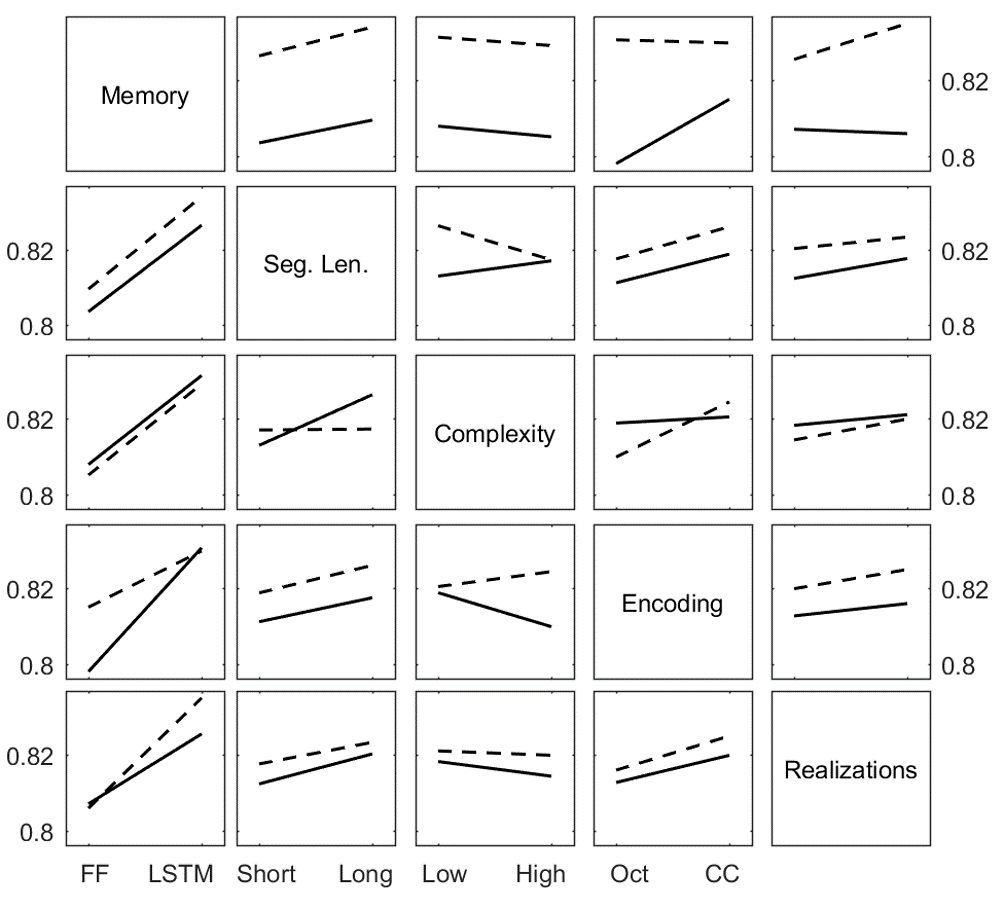
\includegraphics[width=\textwidth]{figures/paper-iii/SuppFigure_2.png}
    \caption[Interaction of different factors and their dependence on accuracy.]{Interaction of different factors and their dependence on accuracy. The IS-RC data was used for this analysis. The solid and dashed lines indicate factors along the rows on levels 1 and 2, respectively.}
    \label{fig:paperiii-suppfigure02}
\end{figure}
The two most important factors that increased prediction accuracy were encoding and memory, while segment length, complexity and number of realizations were less important (\cref{fig:paperiii-suppfigure01}).
The effect of encoding was less prominent in the IS-RC.
Prominent factor interactions include (Supplementary Figure 2): (i) CC encoding models improve with higher complexity, whereas octave encoding models worsen; (ii) increasing segment length positively affects models with low complexity, but does not affect models with a high complexity; and (iii) adding memory improves models with an octave encoding more than models with a CC encoding.
Because the ISRC data are considered the most reliable, we decided to use these data as benchmark for model comparison.
This standard improved as more scorers were added, and the model performance increased (~\cref{fig:paperiii-figure01}a).
The different model configurations described in this section do not represent exhaustive configuration search, and future work experiments might result in improved results.

Figure 2a displays typical scoring outputs (bottom panels) obtained with a single sleep study of the IS-RC cohort in comparison to 6 scorer consensus (top panel).
The model results are displayed as hypnodensity graphs, representing not only discrete sleep stage outputs, but also the probability of occurrence of each sleep state for each epoch (see definition in Data labels, scoring and fuzzy logic section).
As can be seen, all models performed well, and segments of the sleep study with the lowest scorer consensus (top) are paralleled by similar sleep stage probability uncertainty, with performance closest to scoring consensus achieved by an ensemble model described below (second to top).

\subsubsection{Final implementation of automatic sleep scoring algorithm}
Because of model noise, potential inaccuracies and the desire to quantify uncertainty, the final implementation of our sleep
scoring algorithm is an ensemble of different CC models with
small variations in model parameters, such as the number of
feature-maps and hidden nodes.
This was achieved by randomly varying the parameters between 50 and 150\% of the original values using the CC/SH/LS/LSTM as a template (this model achieved similar performance to the CC/LH/LS/LSTM while requiring significantly less computational power).
\begin{table}[]
    \centering
    \caption[STAGES model confusion matrix]{Confusion matrix displaying the relation between different targets and the ensemble estimate. The targets are: Top row – un-weighted consensus. Bottom row – weighted by the scorer agreement at each epoch. The number of analyzed epochs were 53009 (un-weighted) and 36032 (weighted).}
    \label{tab:paperiii-table03}
    \begin{tabular}{@{}llcccccc@{}}
        \toprule
                                           &        & \multicolumn{5}{c}{Target}                    & \multicolumn{1}{l}{} \\ \cline{3-7}
                                           &  & Wake    & N1     & N2      & N3     & REM     & Precision            \\ \midrule
        \multirow{10}{*}{\rotatebox[origin=c]{90}{Model prediction}} & Wake   & 14.08\% & 0.35\% & 0.88\%  & 0.01\% & 0.08\%  & 0.91                 \\
                                           &        & 16.68\% & 0.15\% & 0.44\%  & 0.00\% & 0.02\%  & 0.96                 \\
                                           & N1     & 1.13\%  & 1.78\% & 3.00\%  & 0.00\% & 0.36\%  & 0.28                 \\
                                           &        & 0.47\%  & 0.88\% & 1.15\%  & 0\%    & 0.12\%  & 0.34                 \\
                                           & N2     & 0.29\%  & 0.59\% & 52.58\% & 1.27\% & 0.66\%  & 0.95                 \\
                                           &        & 0.12\%  & 0.25\% & 56.30\% & 0.34\% & 0.32\%  & 0.98                 \\
                                           & N3     & 0.00\%  & 0\%    & 2.13\%  & 4.87\% & 0\%     & 0.7                  \\
                                           &        & 0\%     & 0\%    & 1.09\%  & 4.23\% & 0\%     & 0.91                 \\
                                           & REM    & 0.54\%  & 1.17\% & 0.78\%  & 0\%    & 13.45\% & 0.84                 \\
                                           &        & 0.40\%  & 0.73\% & 0.41\%  & 0\%    & 15.86\% & 0.91                 \\
                                           & Sensitivity       & 0.88    & 0.46   & 0.89    & 0.79   & 0.92    & 0.87                 \\
                                           &        & 0.94    & 0.44   & 0.95    & 0.92   & 0.97    & 0.94                 \\ \bottomrule
    \end{tabular}
\end{table}
All models make errors, but as these errors occur independently of each other, the risk of not detecting and correcting errors falls with increasing model numbers.
For this reason, 16 such models were trained, and at each analyzed segment both mean and variance of model estimates were calculated. 
As expected, the relative model variance (standardized to the average variance in a correct wakefulness prediction) is generally lower in correct predictions (Supplementary Table 3) and this can be used to inform users about uncertain/incorrect estimates. 
To demonstrate the effectiveness of this final implementation, the average of the models is shown alongside the distribution of \plusminus{5234}{14} scorers on 150 epochs, a dataset provided by the AASM (AASM inter-scorer reliability (ISR) dataset, (see Datasets section in Methods). 
On these epochs, the AASM ISR achieved a 90\% agreement between scorers. 
In comparison, the model estimates reached a 95\% accuracy compared to the AASM consensus (Fig. 2b). 
Using the model ensemble and reporting on sleep stage probabilities and inter-model variance for quality purpose constitute the core of our sleep scoring algorithm.
\begin{figure}[tbh]
    \centering
    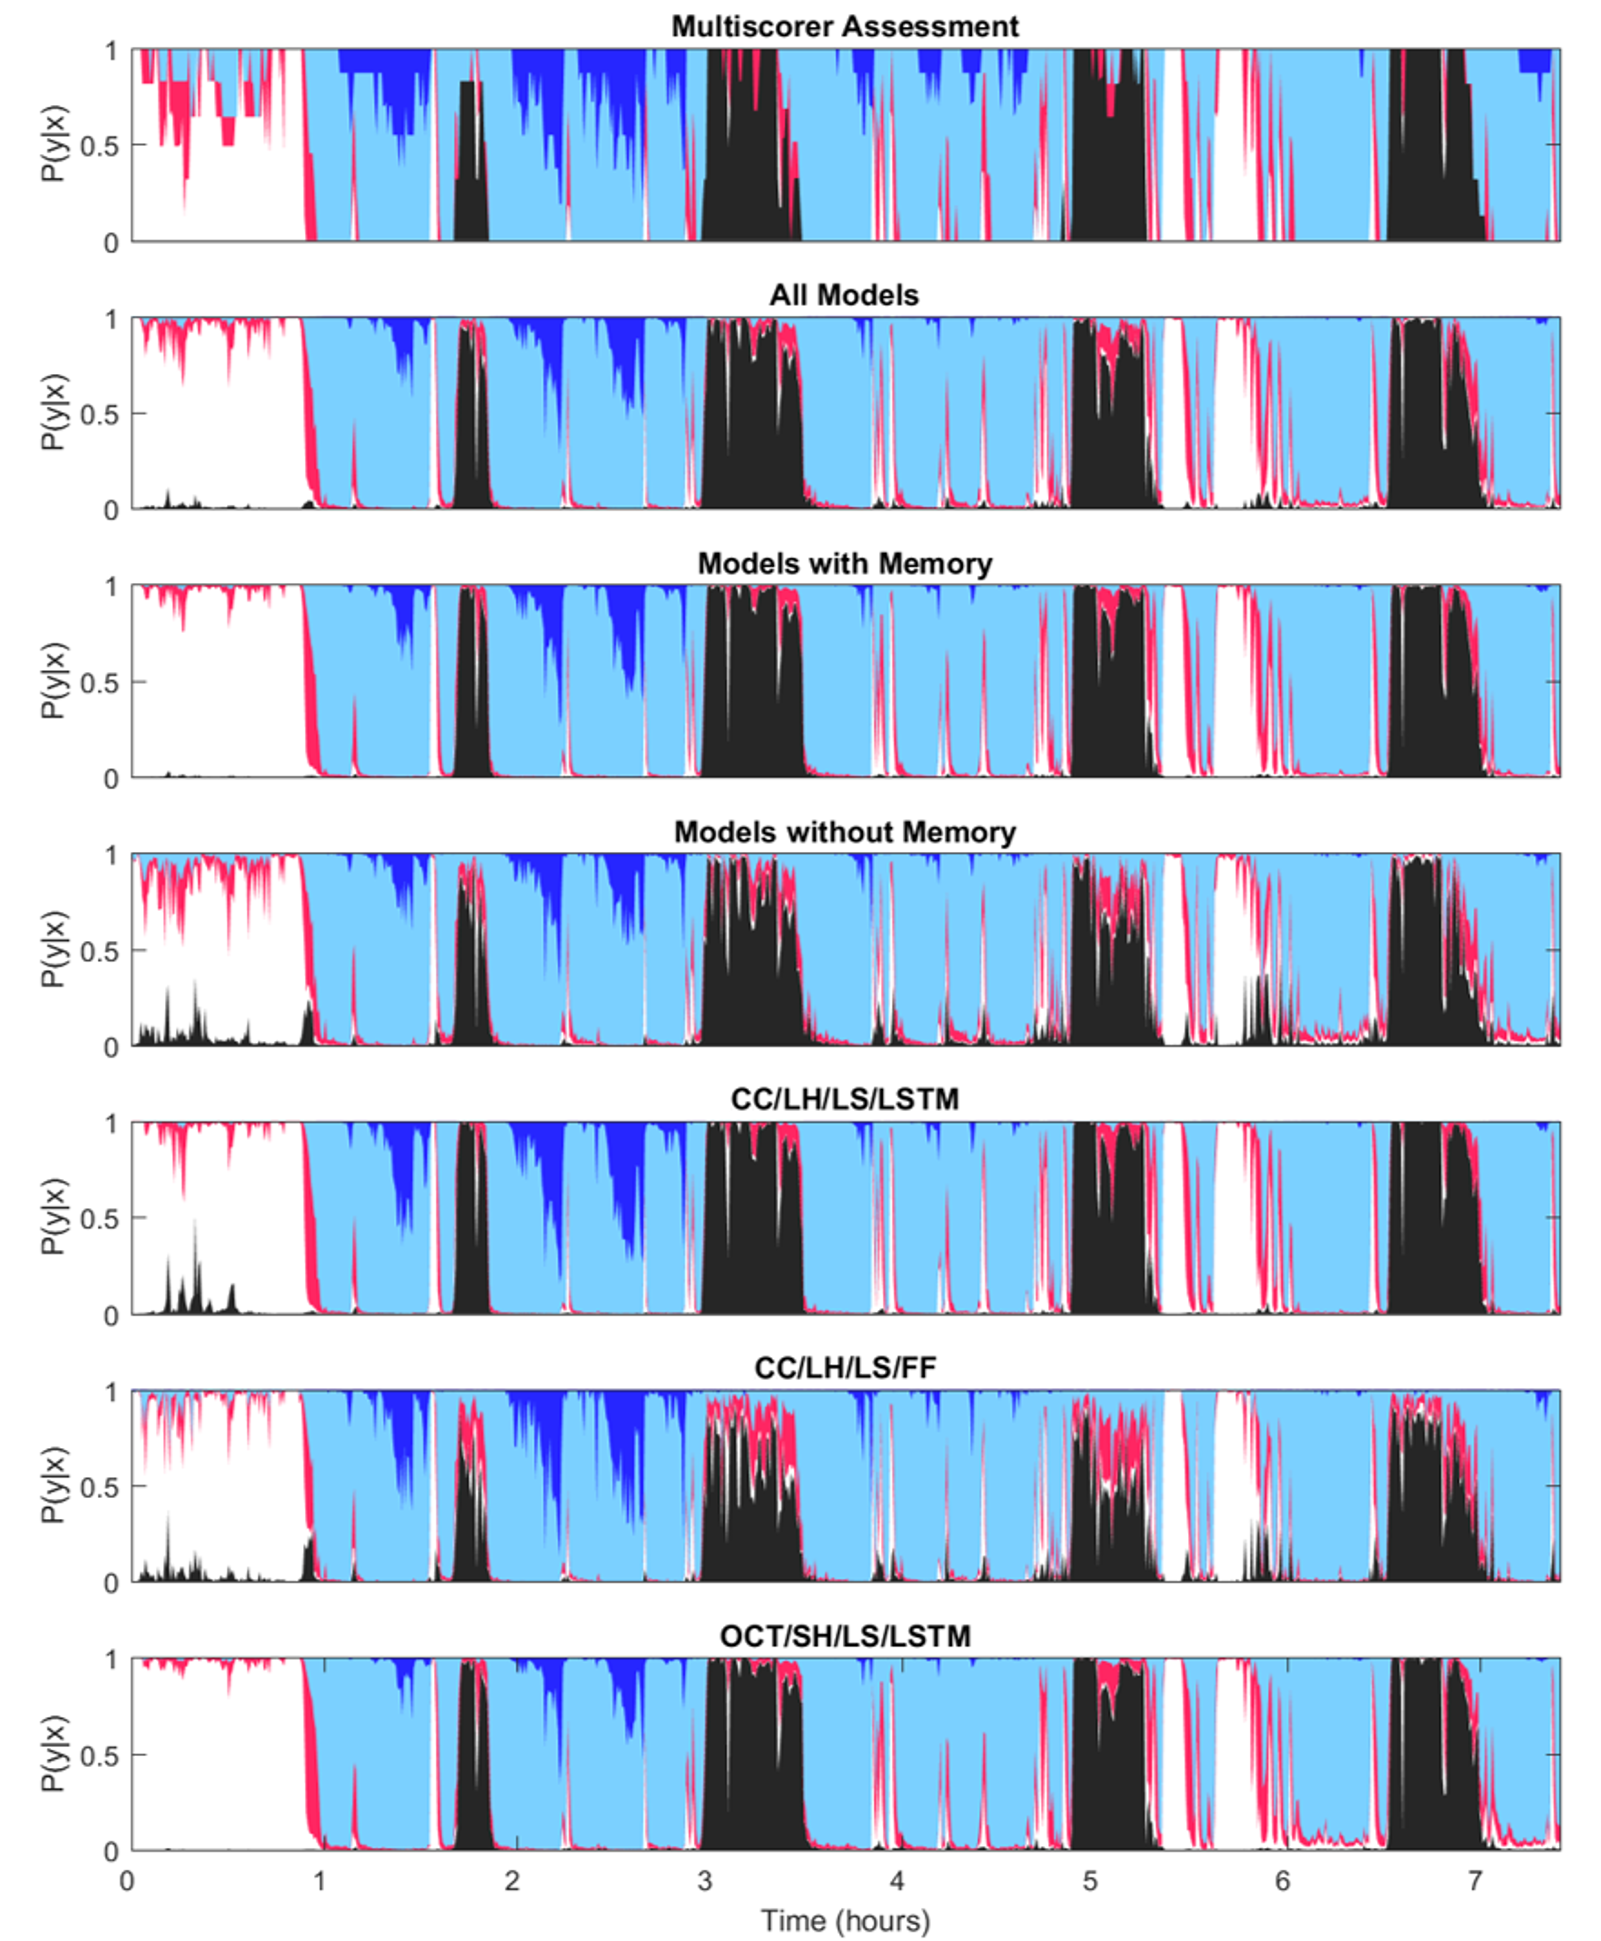
\includegraphics[width=\textwidth]{figures/paper-iii/Figure_2a}
    \caption{The figure displays the hypnodensity graph. Displayed models are, in order: multiple scorer assessment (1); ensembles as described in Supplementary Table 8: All models, those with memory (LSTM) and those without memory (FF) (2–4); single models, as described in Supplementary Table 8 (5–7). OCT is octave encoding, Color codes: white, wake; red, N1; light blue, N2; dark blue, N3; black, REM.}
    \label{fig:paperiii-figure02a}
\end{figure}
\begin{figure}[htb]
    \centering
    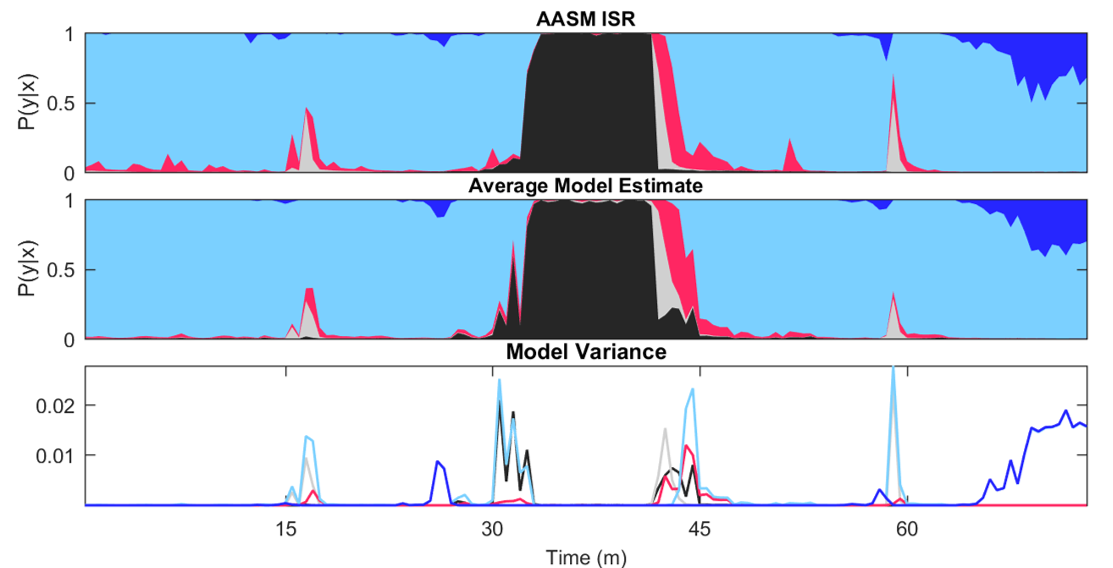
\includegraphics[width=\textwidth]{figures/paper-iii/Figure_2b}
    \caption{The 150 epochs of a recording from the AASM ISR program are analyzed by 16 models with randomly varying parameters, using the CC/SH/LS/LSTM model as a template. These data were also evaluated by \plusminus{5234}{14} different scorers. The distribution of these is shown on top, the average model predictions are shown in the middle, and the model variance is shown at the bottom.}
    \label{fig:paperiii-figure02b}
\end{figure}
\subsubsection{Ensemble/best model performance}
Supplementary Table 2 reports on concordance for our best model, the ensemble of all CC models.
Concordance is presented in a weighted and unweighted manner, between the best model estimate and scorer consensus (\cref{tab:paperiii-table03}).
Weighing of a segment was based on scorer confidence and serves to weigh down controversial segments.
For each recording \textit{i}, the epoch-specific weight $w_n$ and weighted accuracy $\alpha w$ were calculated as:
\begin{align}
\begin{split}
    w_n &= \func{\max_{z \in \mathcal{Z}}}{\func{\mathbf{P}}{\mathbf{y}_n | \mathbf{x}_n}} - \func{\ell_{\mathcal{Z}}^2}{\func{\mathbf{P}}{\mathbf{y}_n | \mathbf{x}_n}}, \\
    \alpha_w^{(i)} &= \frac{1}{\sum_n w_n} \sum_n w_n \! \left( \func{\argmax_{m \in \mathcal{M}}}{\func{\mathbf{P}_m}{\hat{\mathbf{y}}_n | \mathbf{x}_n}} \cap \func{\argmax_{z \in \mathcal{Z}}}{\func{\mathbf{P}_z}{\mathbf{y}_n | \mathbf{x}_n}} \right),
\end{split}
\end{align}
where $\func{\ell_{\mathcal{Z}}^2}{\func{\mathbf{P}}{\mathbf{y}_n | \mathbf{x}_n}}$ is the second most likely stage assessed by the set of scorers (experts) denoted by $\mathcal{Z}$, of the \textit{n}th epoch in a sleep recording.
As with scorers, the biggest discrepancies occurred between wake versus N1, N1 versus N2 and N2 versus N3.
Additionally, the weighted performance was almost universally better than the unweighted performance, raising overall accuracy from 87 to 94\%, indicating a high consensus between automatic scoring and scorers in places with high scorer confidence.
An explanation for these results could be that both scorers and model are forced to make a choice between two stages when data are ambiguous.
An example of this may be seen in Fig. 2a.
Between 1 and 3 h, several bouts of N3 occur, although they often do not reach the threshold for being the most likely stage
As time progresses, more evidence for N3 appears reflecting increased proportion of slow waves per epoch, and confidence increases, which finally yields “definitive” N3. 
This is seen in both model and scorer estimates.
Choosing to present the data as hypnodensity graphs mitigates this problem. 
The various model estimates produce similar results, which also resemble the scorer assessment distribution, although models without memory fluctuate slightly more, and tend to place a higher probability on REM sleep in periods of wakefulness, since no contextual information is provided

% \begin{figure}[!tb]
%     \myfloatalign   
%     \subfloat[]
%     {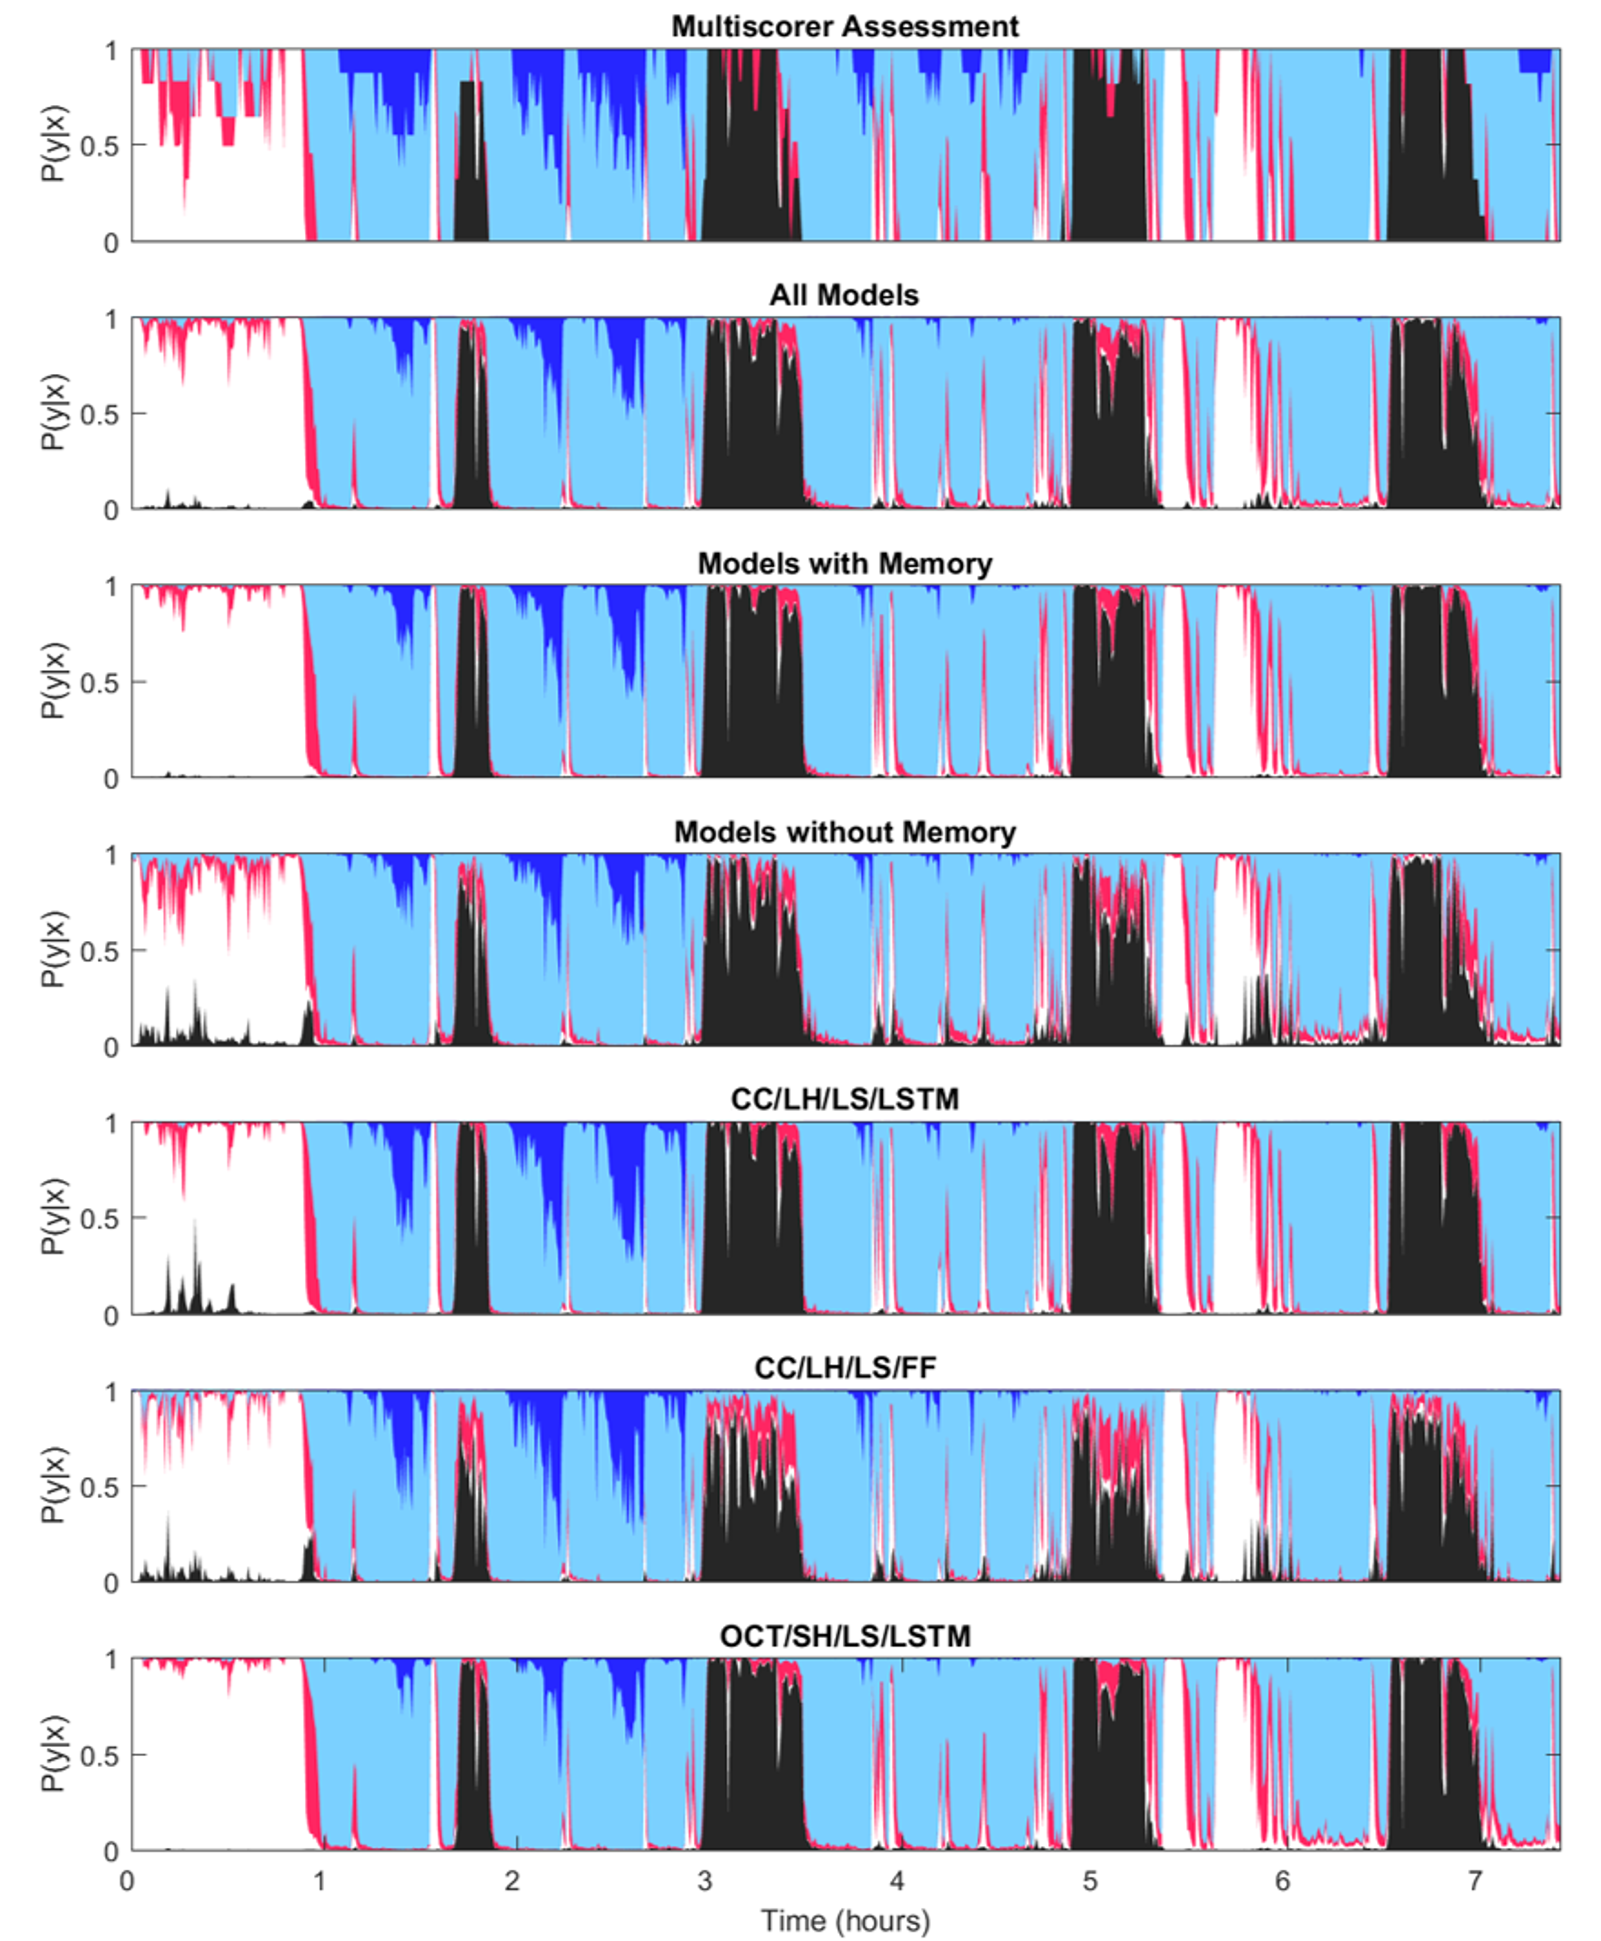
\includegraphics[width=\textwidth]{figures/paper-iii/Figure_2a}} \\
%     \subfloat[]
%     {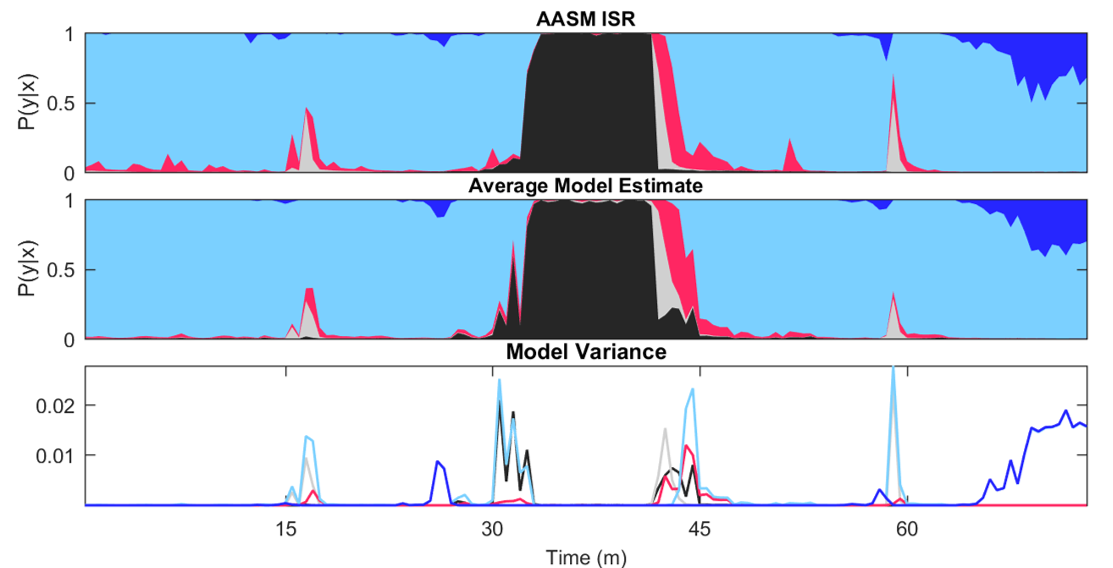
\includegraphics[width=\textwidth]{figures/paper-iii/Figure_2b}}
%     \caption[Hypnodensity example evaluated by multiple scorers and different predictive models]{Hypnodensity example evaluated by multiple scorers and different predictive models. (a)  b }
%     \label{fig:paperiii-figure02}
% \end{figure}

\subsubsection{Influences of sleep pathologies}
As seen in Table 2, the different cohorts achieve different performances.
To see how much may be attributed to various pathologies, five different analyses of variance were made, with accuracy as the dependent variable, using cohort, age (grouped as age $<$ 30, 30 $\leq$ age $<$ 50, and age $\geq$ 50) and sex as covariates (Supplementary Table 4), investigating the effect of insomnia, OSA, restless leg syndrome (RLS), periodic leg movement index (PLMI) and T1N on accuracy of our machine learning routine versus human scoring. 
This was performed in the cohort mentioned above with addition of the Austrian Hypersomnia Cohort (AHC)35. 
The \textit{p}-values obtained from paired \textit{t}-testing for each condition were $0.75$ (insomnia), $7.53 \times 10^{-4}$ (OSA), $0.13$ (RLS), $0.22$ (PLMI) and $1.77 \times 10^{-15}$ (T1N) respectively, indicating that only narcolepsy had a strong effect on scorer performance. 
Additionally, in the context of narcolepsy, cohort and age yielded \textit{p}-values between $3.69 \times 10^{-21}$ and $2.81 \times 10^{-82}$ and between $0.62$ and $6.73 \times 10^{-6}$, respectively. 
No significant effect of gender was ever noted. 
Cohort effects were expected and likely reflect local scorer performances and differences in PSG hardware and filter setups at every site. 
Decreased performance with age likely reflects decreased EEG amplitude, notably in N3/slow wave sleep amplitude with age36.

\begin{figure}[tb]
    \myfloatalign   
    \subfloat[]
    {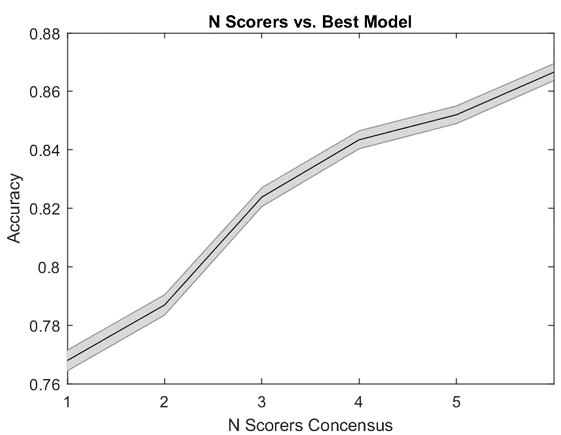
\includegraphics[width=0.48\textwidth]{figures/paper-iii/Figure_1a}}  ~
    \subfloat[]
    {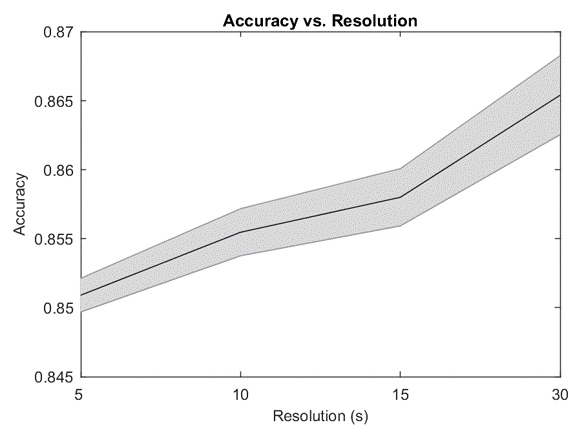
\includegraphics[width=0.5 \textwidth]{figures/paper-iii/Figure_1b}}
    \caption[Accuracy per scorer and by time resolution]{Accuracy per scorer and by time resolution. (a) The effect on scoring accuracy as golden standard is improved. Every combination of $N$ scorers is evaluated in an unweighted manner and the mean is calculated. Accuracy is shown with mean (solid black line) and a 95\% confidence interval (gray area). (b) Predictive performance of best model at different resolutions. Performance is shown as mean accuracy (solid black line) with a 95\% confidence interval
(gray area).}
    \label{fig:paperiii-figure01}
\end{figure}
\subsubsection{Resolution of sleep stage scoring}
Epochs are evaluated with a resolution of 30 s, a historical standard that is not founded in anything physiological, and limits the analytical possibilities of a hypnogram.
Consequently, it was examined to what extent the performance would change as a function of smaller resolution.
Only the models using a segment size of 5 s were considered.
Segments were averaged to achieve performances at 5, 10, 15 and 30 s resolutions, and the resulting performances in terms of accuracy are shown in~\cref{fig:paperiii-figure01}b. 
Although the highest performance was found using a resolution of 30 s, performance dropped only slightly with decreasing window sizes.

\subsection{Discussion}
In recent years, machine learning has been used to solve similar or more complex problems, such as labeling images, understanding speech and translating language, and have seen advancement to the point where humans are now sometimes outperformed21–23, while also showing promising results in various medical fields24–29.
Automatic classification of sleep stages using automatic algorithms is not novel44,45, but only recently has this type of machine learning been applied and the effectiveness has only been demonstrated in a small numbers of sleep studies46–49. 
Because PSGs contain large amounts of manually annotated “gold standard” data, we hypothesized this method would be ideal to
automatize sleep scoring.
We have shown that machine learning can be used to score sleep stages in PSGs with high accuracy in multiple physical locations in various recording environments, using different protocols and hardware/software configurations, and in subjects with and without various sleep disorders.

After testing various machine learning algorithms with and without memory and specific encodings, we found increased robustness using a consensus of multiple algorithms in our prediction.
The main reason for this is likely the sensitivity of each algorithm to particular aspects of each individual recording, resulting in increased or decreased predictability.
\Cref{fig:paperiii-suppfigure01}b displays the correlations between different models.
Models that incorporate an ensemble of different models generally have a higher overall correlation coefficient than singular models, and since individual models achieve similar performances, it stands to reason that these would achieve the highest performance.

One potential source for this variability was, in addition to the stochastic nature of the training, the fact recordings were conducted in different laboratories that were using different hardware and filters, and had PSGs scored by technicians of various abilities.
Another contributor was the presence of sleep pathologies in the dataset that could influence machine learning.
Of the pathologies tested, only narcolepsy had a very significant effect on the correspondence between manual and machine learning methods ($p=1.77 \times 10^{-15}$ vs $p=7.53 \times 10^{-4}$ for sleep apnea for example, see Supplementary Tables 4 and 7).
This was not surprising as the pathology is characterized by unusual sleep stage transitions, for example, transitions from wake to REM sleep, which may make human or machine learning staging more difficult.
This result suggests that reporting inter-model variations in accuracy for each specific patient has value in flagging unusual sleep pathologies, so this metric is also reported by our detector.

Unlike previous attempts using automatic detector validations, we were able to include 70 subjects scored by 6 technicians in different laboratories (the IS-RC cohort)31 to independently validate our best automatic scoring consensus algorithm.
This allowed us to estimate the performance at 87\% in comparison to the performance of a consensus score for every epoch among six expert technicians (ultimate gold standard) (Table 1).
Including more scorers produces a better gold standard, and as~\cref{fig:paperiii-figure01}a indicates, the model accuracy also increases with more scorers.
Naturally, extrapolating from this should be done with caution; however, it is reasonable to assume that the accuracy would continue to increase with increased scorers.
In comparison, performance of any individual scorer ranges from 74 to 85\% when compared to the same six-scorer gold standard, keeping in mind this performance is artificially inflated since the same scorers evaluated are included in the gold standard (unbiased performance of any scorer versus consensus of remaining 5 scorers range from 69 to 80\%). 
The best model achieves 87\% accuracy using 5 scorers (~\cref{fig:paperiii-figure01}a and Table 1), and is statistically higher than all scorers.

As with human scorers, the biggest discrepancies in machine learning determination of sleep stages occurred between wake versus N1, N1 versus N2 and N2 versus N3.
This is logical as these particular sleep stage transitions are part of a continuum, artificially defined and subjective. To give an example: an epoch comprised of 18\% slow wave activity is considered N2 while an epoch comprised of 20\% slow wave activity qualifies as N3.
Overall, data indicate that our machine learning algorithm performs better than individual scorers, as typically used in clinical practice, or similar to the best of 5 scorers in comparison to a combination of 5 experts scoring each epoch by consensus.
It is also able to score at higher resolution, i.e., 5 s, making it unnecessary to score sleep stages by 30 s epochs, an outdated rule dating from the time sleep was scored on paper. 
Although the data sample used for multi-scorer validation contained only female subjects, the scoring accuracy of our model was not seen to be affected by gender (Supplementary Table 3) in another analysis.

Using our models, and considering how typical T1N behaved in our sleep stage machine learning routines, we extracted features that could be useful to diagnose this condition.
T1N ischaracterized by the loss of hypocretin-producing cells in the hypothalamus3 and can be best diagnosed by measuring hypocretin levels in the CSF11, a procedure that requires a lumbar puncture, a rarely performed procedure in the United States. 
At the symptomatic level, T1N is characterized by sleepiness, cataplexy (episodes of muscle weakness during wakefulness triggered by emotions) and numerous symptoms reflecting poor nocturnal sleep (insomnia) and symptoms of “dissociated REM sleep”.
Dissociated REM sleep is reflected by the presence of unusual states of consciousness where REM sleep is intermingled with wakefulness, producing disturbing reports of dreams that interrupt wakefulness and seem real (dream-like hallucinations), or episodes where the sleeper is awake but paralyzed as in normal REM sleep (sleep paralysis).
The current gold standard for T1N diagnosis is the presence of cataplexy and a positive MSLT.
In a recent large study of the MSLT, specificity and sensitivity for T1N was 98.6\% and 92.9\% in comparing T1N versus controls, and 71.2\% and 93.4\% in comparing T1N versus other hypersomnia cases (high pretest probability cohort)10.

Table 4 and Supplementary Table 5 reveal features found in nocturnal PSGs that discriminate type 1 narcoleptics and nonnarcoleptics.
One of the most prominent features, short latency REM sleep, bears great resemblance to the REM sleep latency, which is already used clinically to diagnose narcolepsy, although in this case it is calculated using fuzzy logic and thus represent a latency where accumulated sleep is suggestive of a high probability of REM sleep having occurred (as opposed to a discreteREM latency scored by a technician).
A short REM  latency during nocturnal PSG (typically 15 min) has recently been shown to be extremely specific (99\%) and moderately sensitive (40–50\%) for T1N10,50.
The remaining selected features also describe a generally altered sleep architecture, particularly between REM sleep,
light sleep and wake, aspects of narcolepsy already known and
thus reinforcing their validity as biomarkers.

For example, the primary feature as determined by the RFE algorithm was the time taken until 5\% of the accumulated sum of the probability products between stages W, N2 and REM had been reached (see also Table 4), which reflects the uncertainty between wakefulness, REM and N2 sleep at the beginning of the night.
Specifically, for the \textit{n}th epoch, the model will output probabilities for each sleep stage, and the proto-feature $\boldsymbol{\Phi}_n$ is calculated as
\begin{equation}
    \boldsymbol{\Phi}_n = \func{p}{\wake} \times \func{p}{\nII} + \func{p}{\wake} \times \func{p}{\rem} + \func{p}{\nII} \times \func{p}{\rem}.
\end{equation}
The feature value is then calculated as the time it takes in minutes for the accumulated sum of $\boldsymbol{\Phi}_n$ to reach 5\% of the total sum $\sum_n \boldsymbol{\Phi}_n$.
Since each of probability product in $\boldsymbol{\Phi}_n$ reflects the staging uncertainty between each sleep stage pair, $\boldsymbol{\Phi}_n$ alone reflects the general sleep stage uncertainty for that specific epoch as predicted by the model.
A very high value will be attained for epoch $n$ if the probabilities for N2, W and REM are equally probable with probabilities for the remaining sleep stages being low or close to zero. 
A PSG with a high staging uncertainty between sleep and wake early in the night would reach the 5\% threshold rapidly.

Using these features, we were able to determine an optimal cutoff that discriminated narcolepsy from controls and any other patients with as high specificity and sensitivity as the MSLT (Supplementary Table 6), notably when HLA typing is added.
This is true for both the test and the never seen replication samples.
Although we do observe a small drop in specificity in the replication sample, the efficacy of the detector was also tested in the context of naive patients with hypersomnia (high pretest probability sample), and performance found to be similar to the MSLT.

MSLT testing requires that patients spend an entire night and day in a sleep laboratory.
The use of this novel biomarker could reduce time spent to a standard 8 h night recording, as done for the screening of other sleep pathologies (e.g., OSA), allowing improved recognition of T1N cases at a fraction of the cost.
A positive predictive value could also be provided depending on the nature of the sample and known narcolepsy prevalence (low in general population screening, intermediary in overall clinic population sample and high in hypersomnia cohorts). 
It also opens the possibility of using home sleep recordings for diagnosing narcolepsy. 
In this direction, because of the probabilistic and automatic nature of our biomarker, estimates from more than one night could be automatically analyzed and combined over time, ensuring improved prediction.
However, it is important to note that this algorithm will not replace the MSLT in the ability to predict excessive daytime sleepiness through the measure of mean sleep latency across daytime naps, which is an important characteristic of other hypersomnias.

In conclusion, models which classify sleep by assigning a membership function to each of five different stages of sleep for each analyzed segment were produced, and factors contributing to the performance were analyzed. 
The models were evaluated on different cohorts, one of which contained 70 subjects scored by 6 different sleep scoring technicians, allowing for inter-scorer reliability assessments.
The most successful model, consisting of an ensemble of different models, achieved an accuracy of 87\% on this dataset, and was statistically better performing than any individual scorer.
It was also able to score sleep stages with high accuracy at lower time resolution (5 s), rendering the need for scoring per 30 s epoch obsolete.
When predictions were weighted by the scorer agreement, performance rose to 95\%, indicating a high consensus between the model and human scorers in areas of high scorer agreement.
A final implementation was made using an ensemble with small variations of the best single model.
This allowed for better predictions, while also providing a measure of uncertainty in an estimate.

When the staging data were presented as hypnodensity distributions, the model conveyed more information about the subject than through a hypnogram alone.
This led to the creation of a biomarker for narcolepsy that achieved similar performance to the current clinical gold standard, the MSLT, but only requires a single sleep study.
If increased specificity is needed, for example, in large-scale screening, HLA or additional genetic typing brings specificity above 99\% without loss of sensitivity.
This presents an option for robust, consistent, inexpensive and simpler diagnosis of subjects who may have narcolepsy, as such tests may also be carried out in a home environment.

This study shows how hypnodensity graphs can be created automatically from raw sleep study data, and how the resulting interpretable features can be used to generate a diagnosis probability for T1N.
Another approach would be to classify narcolepsy directly from the neural network by optimizing the performance not only for sleep staging, but also for direct diagnosis by adding an additional softmax output, thereby creating a multitask classifier.
This approach could lead to better predictions, since features are not then limited to by a designer imagination. 
A drawback of this approach is that features would no longer be as interpretable and meaningful to clinicians. 
If meaning could be extracted from these neural network generated features, this might open the door to a single universal sleep analysis model, covering multiple diseases.
Development of such a model would require adding more subjects with narcolepsy and other conditions to the pool of training data.

% \section{Sleep stage classification algorithms}
